\documentclass[10pt]{article}
\usepackage[utf8]{inputenc}
\usepackage{geometry}
\usepackage[sort]{natbib}
\usepackage{pxfonts}
\usepackage{graphicx}
\usepackage{setspace}
\usepackage{hyperref}
\usepackage{lineno}
\usepackage{authblk}
\usepackage{pdflscape}
\usepackage{rotating}

\doublespacing
\linenumbers

\title{\textit{Supplementary materials for:} Fitness tracking reveals task-specific associations between
  memory, mental health, and exercise}
\author[1, $\star$]{Jeremy R. Manning}
\author[1,2]{Gina M. Notaro}
\author[1]{Esme Chen}
\author[1]{Paxton C. Fitzpatrick}
\affil[1]{Dartmouth College, Hanover, NH}
\affil[2]{Lockheed Martin, Bethesda, MD}
\affil[$\star$]{Address correspondence to jeremy.r.manning@dartmouth.edu}

\begin{document}
\maketitle

\renewcommand{\thefigure}{S\arabic{figure}}


\begin{figure}[p]
\centering
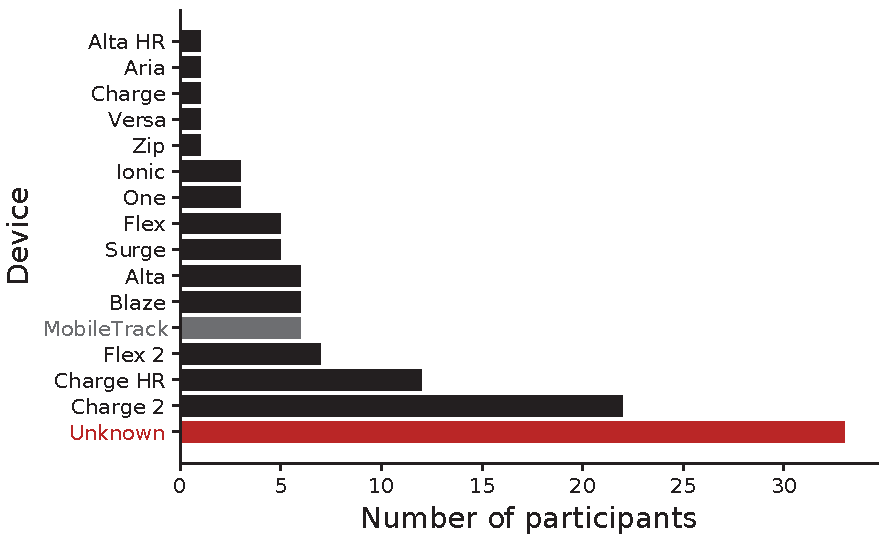
\includegraphics[width=0.6\textwidth]{figs/devices}
\caption{\textbf{Fitbit devices.}  The bars indicate the numbers of
  participants whose fitness tracking data came from each model of
  Fitbit device.  ``MobileTrack'' refers to participants who used
  smartphone accelerometer information to track their activity via the
  Fitbit smartphone app.
  ``Unknown''  denotes participants whose device information was not
  available from their available Fitbit data.}
\label{fig:devices}
\end{figure}


\begin{sidewaysfigure}[p]
\centering
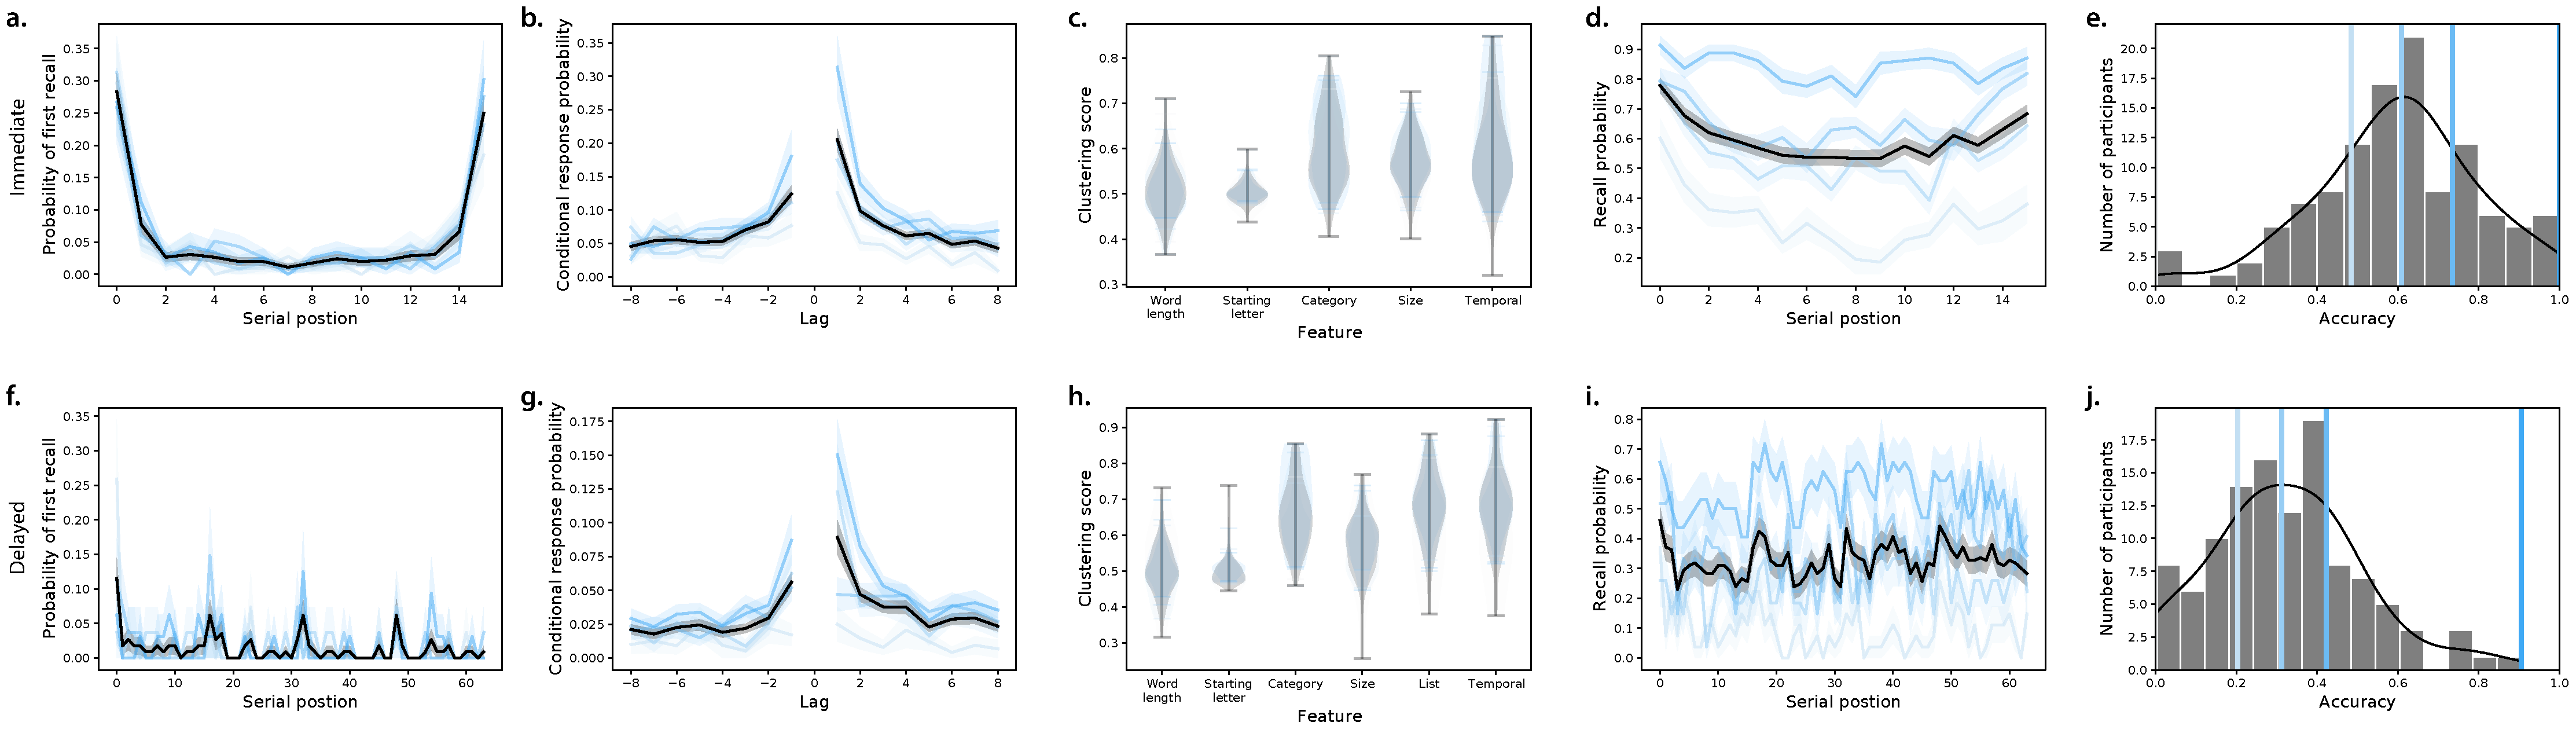
\includegraphics[width=1\textwidth]{figs/free_recall_behavior}
\caption{\textbf{Free recall behavioral results.}}
\label{fig:fr_behavioral}
\end{sidewaysfigure}

\begin{sidewaysfigure}[p]
\centering
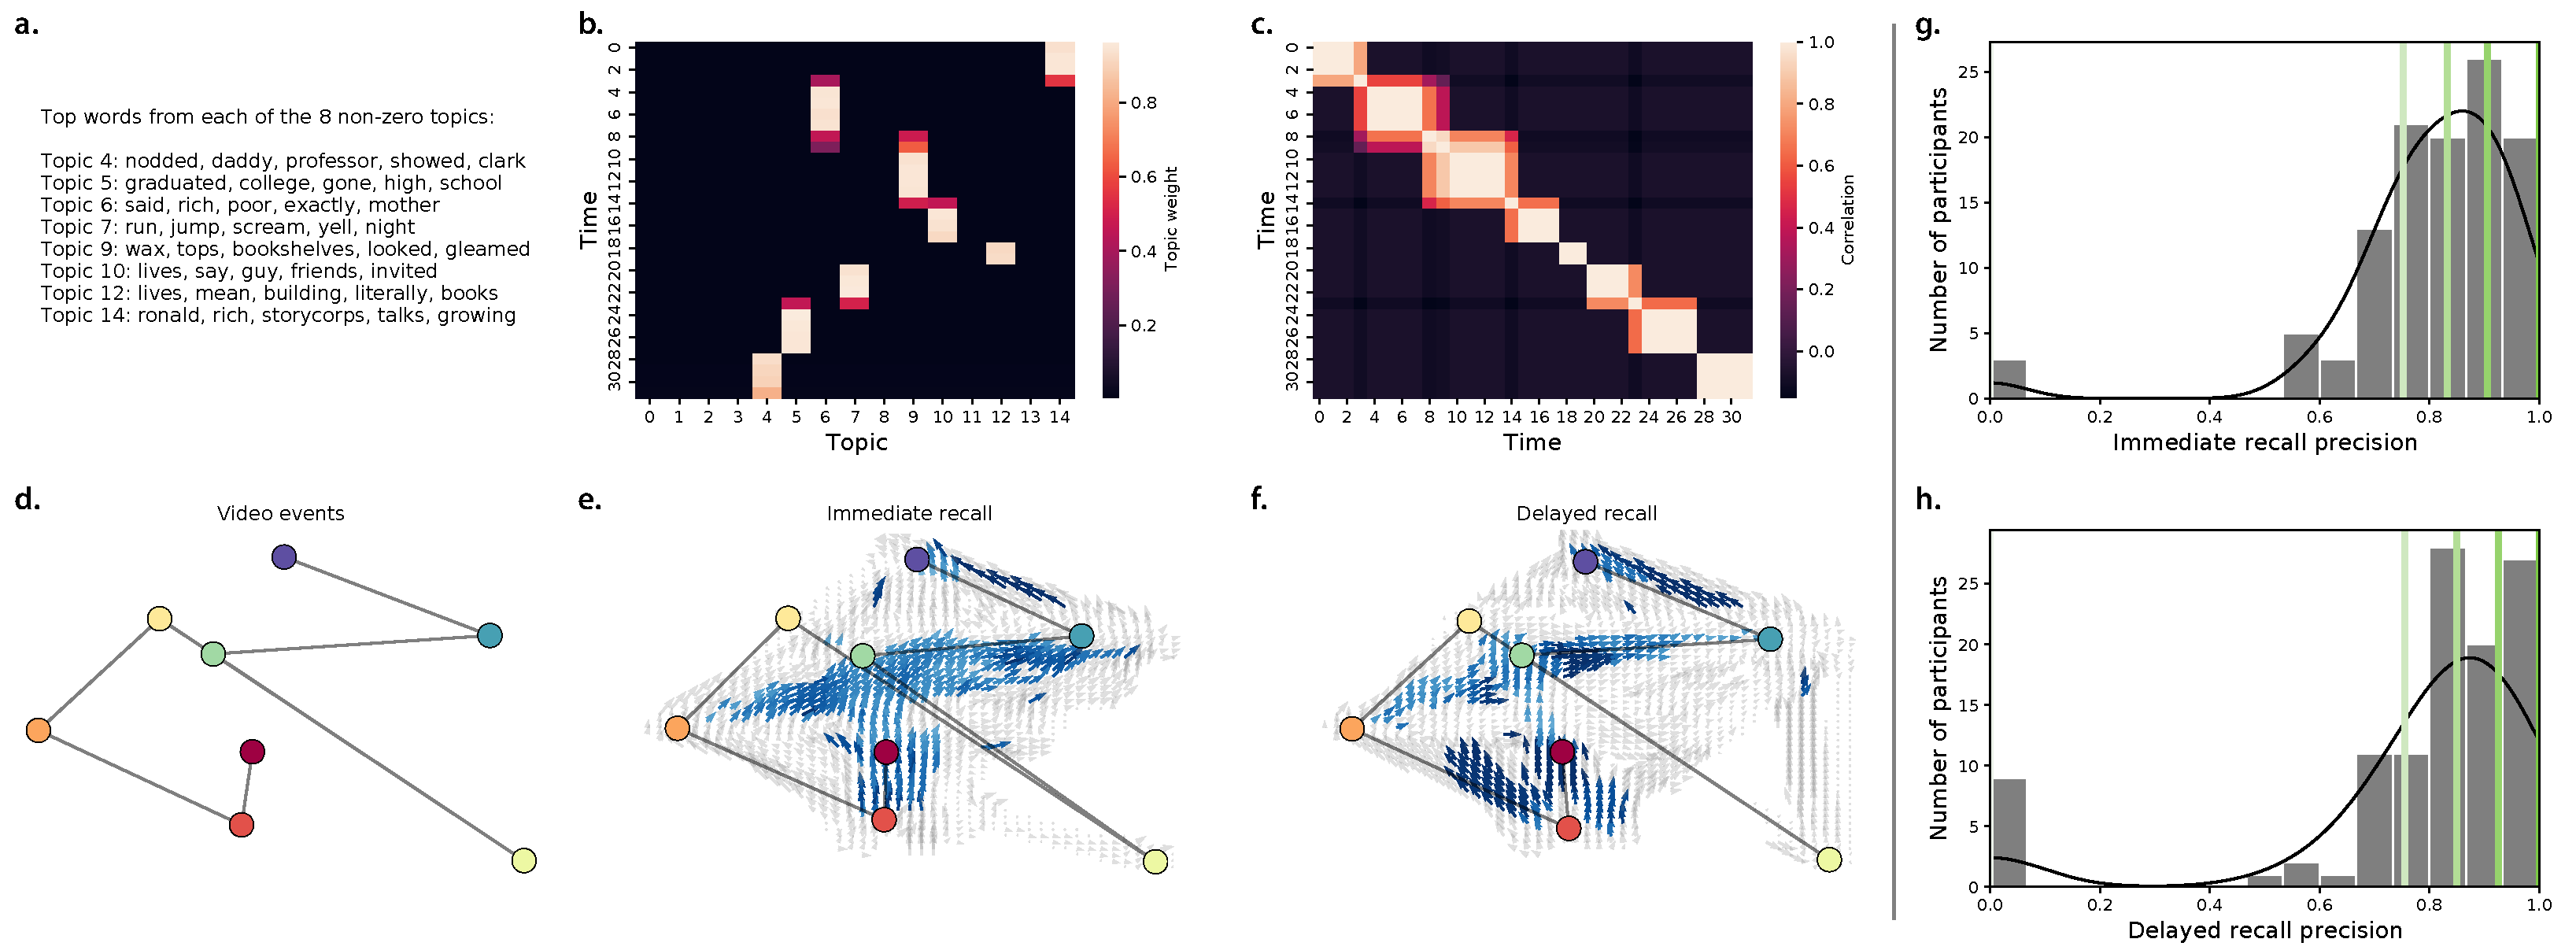
\includegraphics[width=1\textwidth]{figs/naturalistic_recall_behavior}
\caption{\textbf{Naturalistic recall behavioral results.}}
\label{fig:nat_behavioral}
\end{sidewaysfigure}

\begin{figure}[p]
\centering
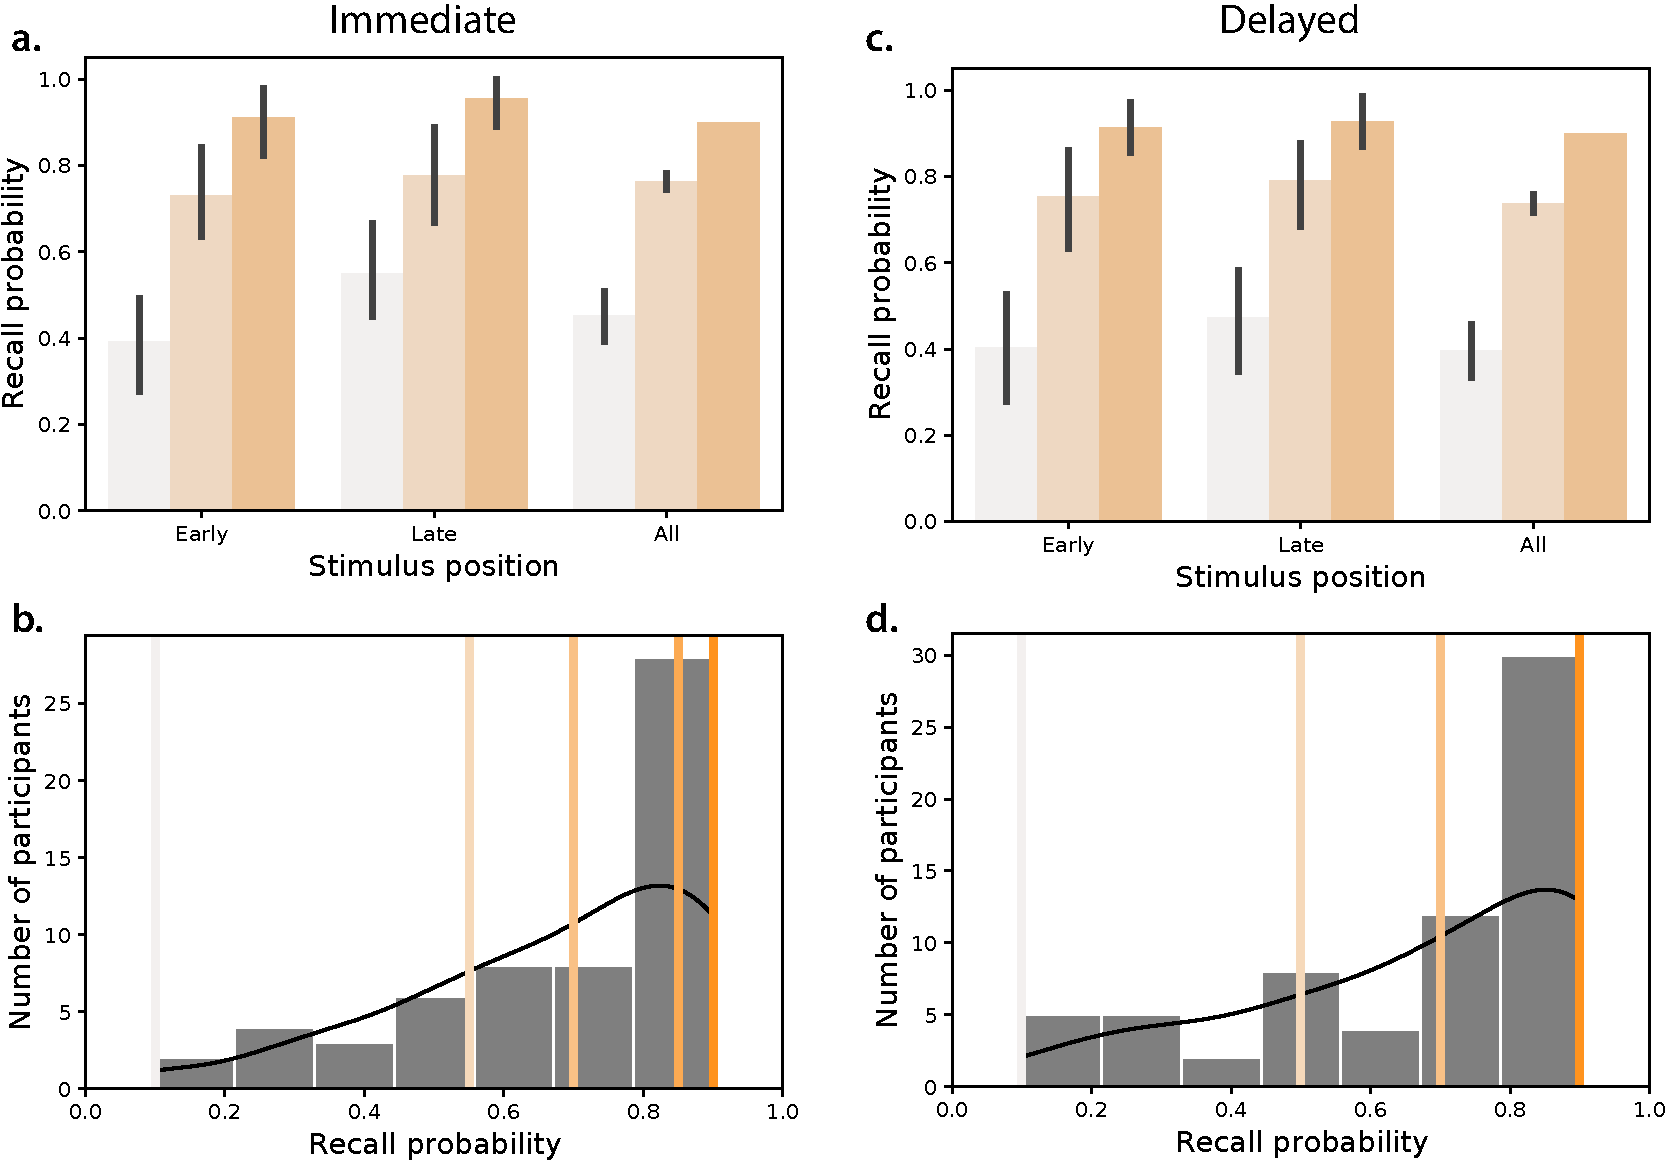
\includegraphics[width=0.6\textwidth]{figs/vocab_learning_behavior}
\caption{\textbf{Foreign language vocabulary learning behavioral results.}}
\label{fig:vocab_behavioral}
\end{figure}

\begin{figure}[p]
\centering
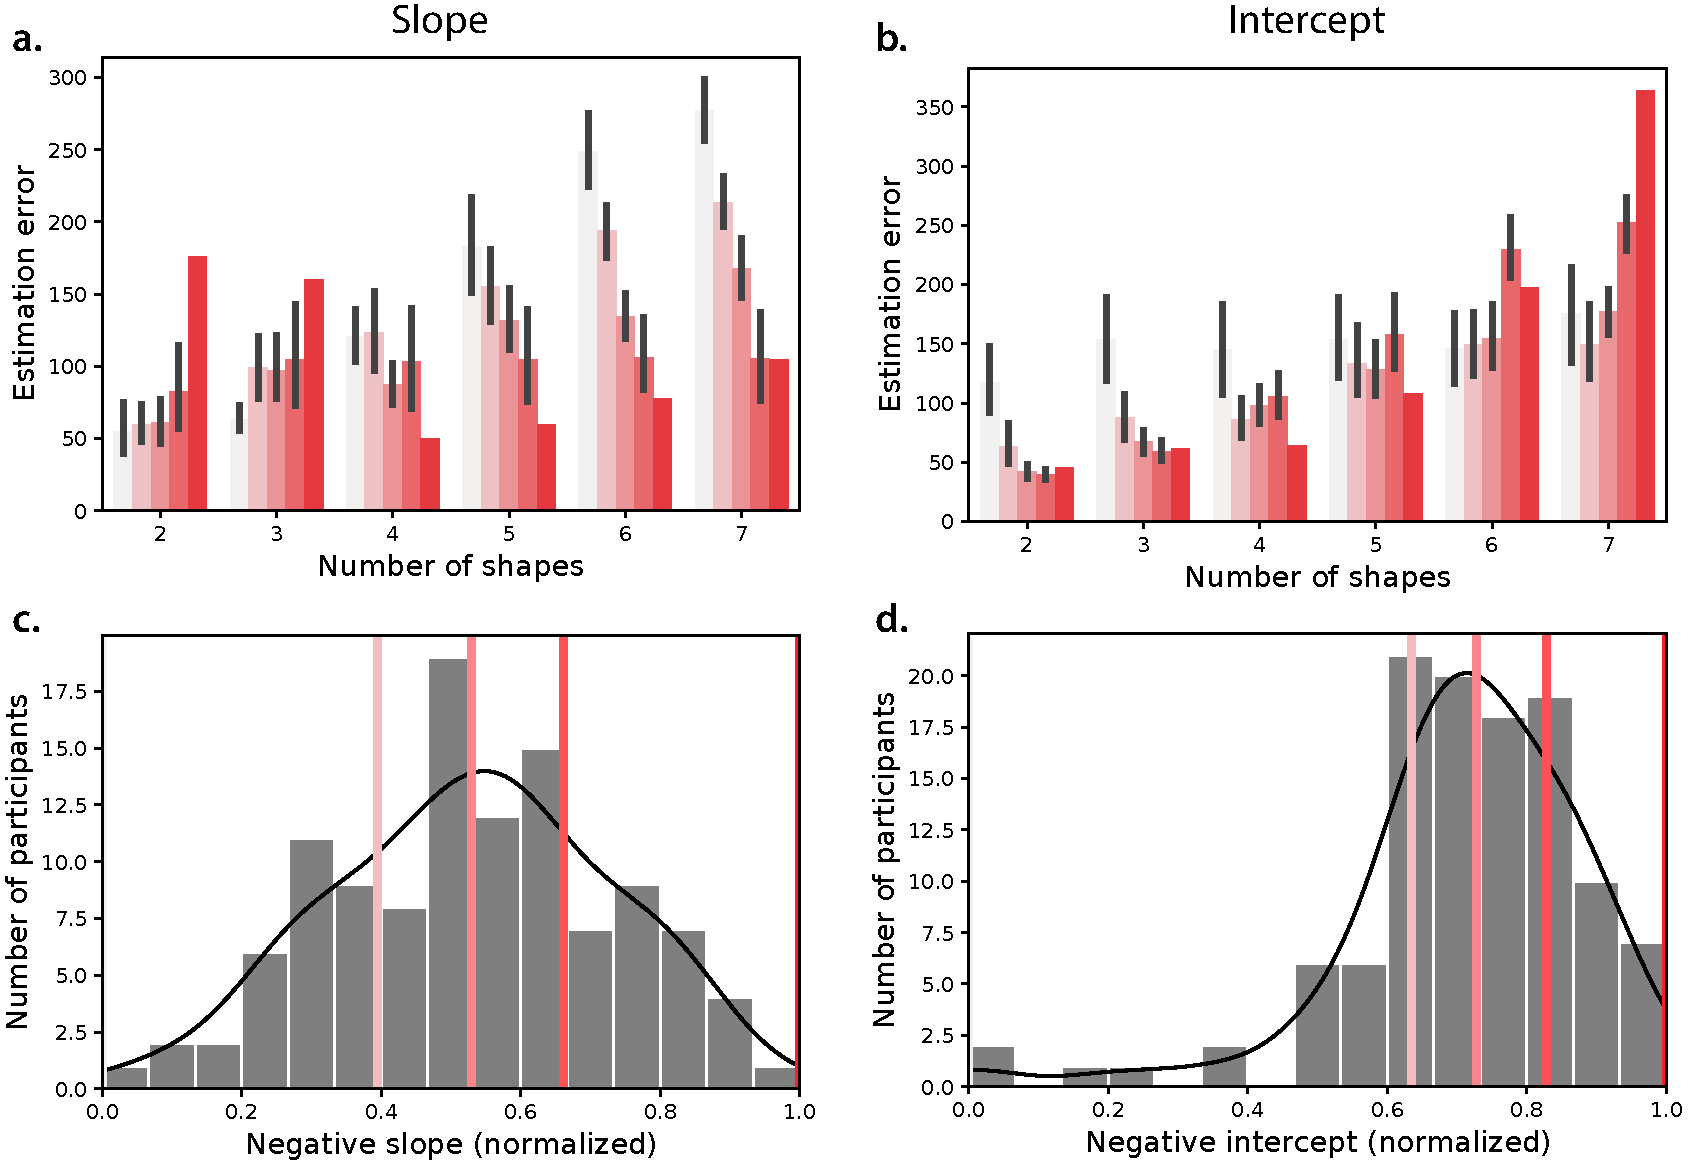
\includegraphics[width=0.6\textwidth]{figs/spatial_learning_behavior}
\caption{\textbf{Spatial learning behavioral results.}}
\label{fig:spatial_behavioral}
\end{figure}

\begin{sidewaysfigure}[p]
\centering
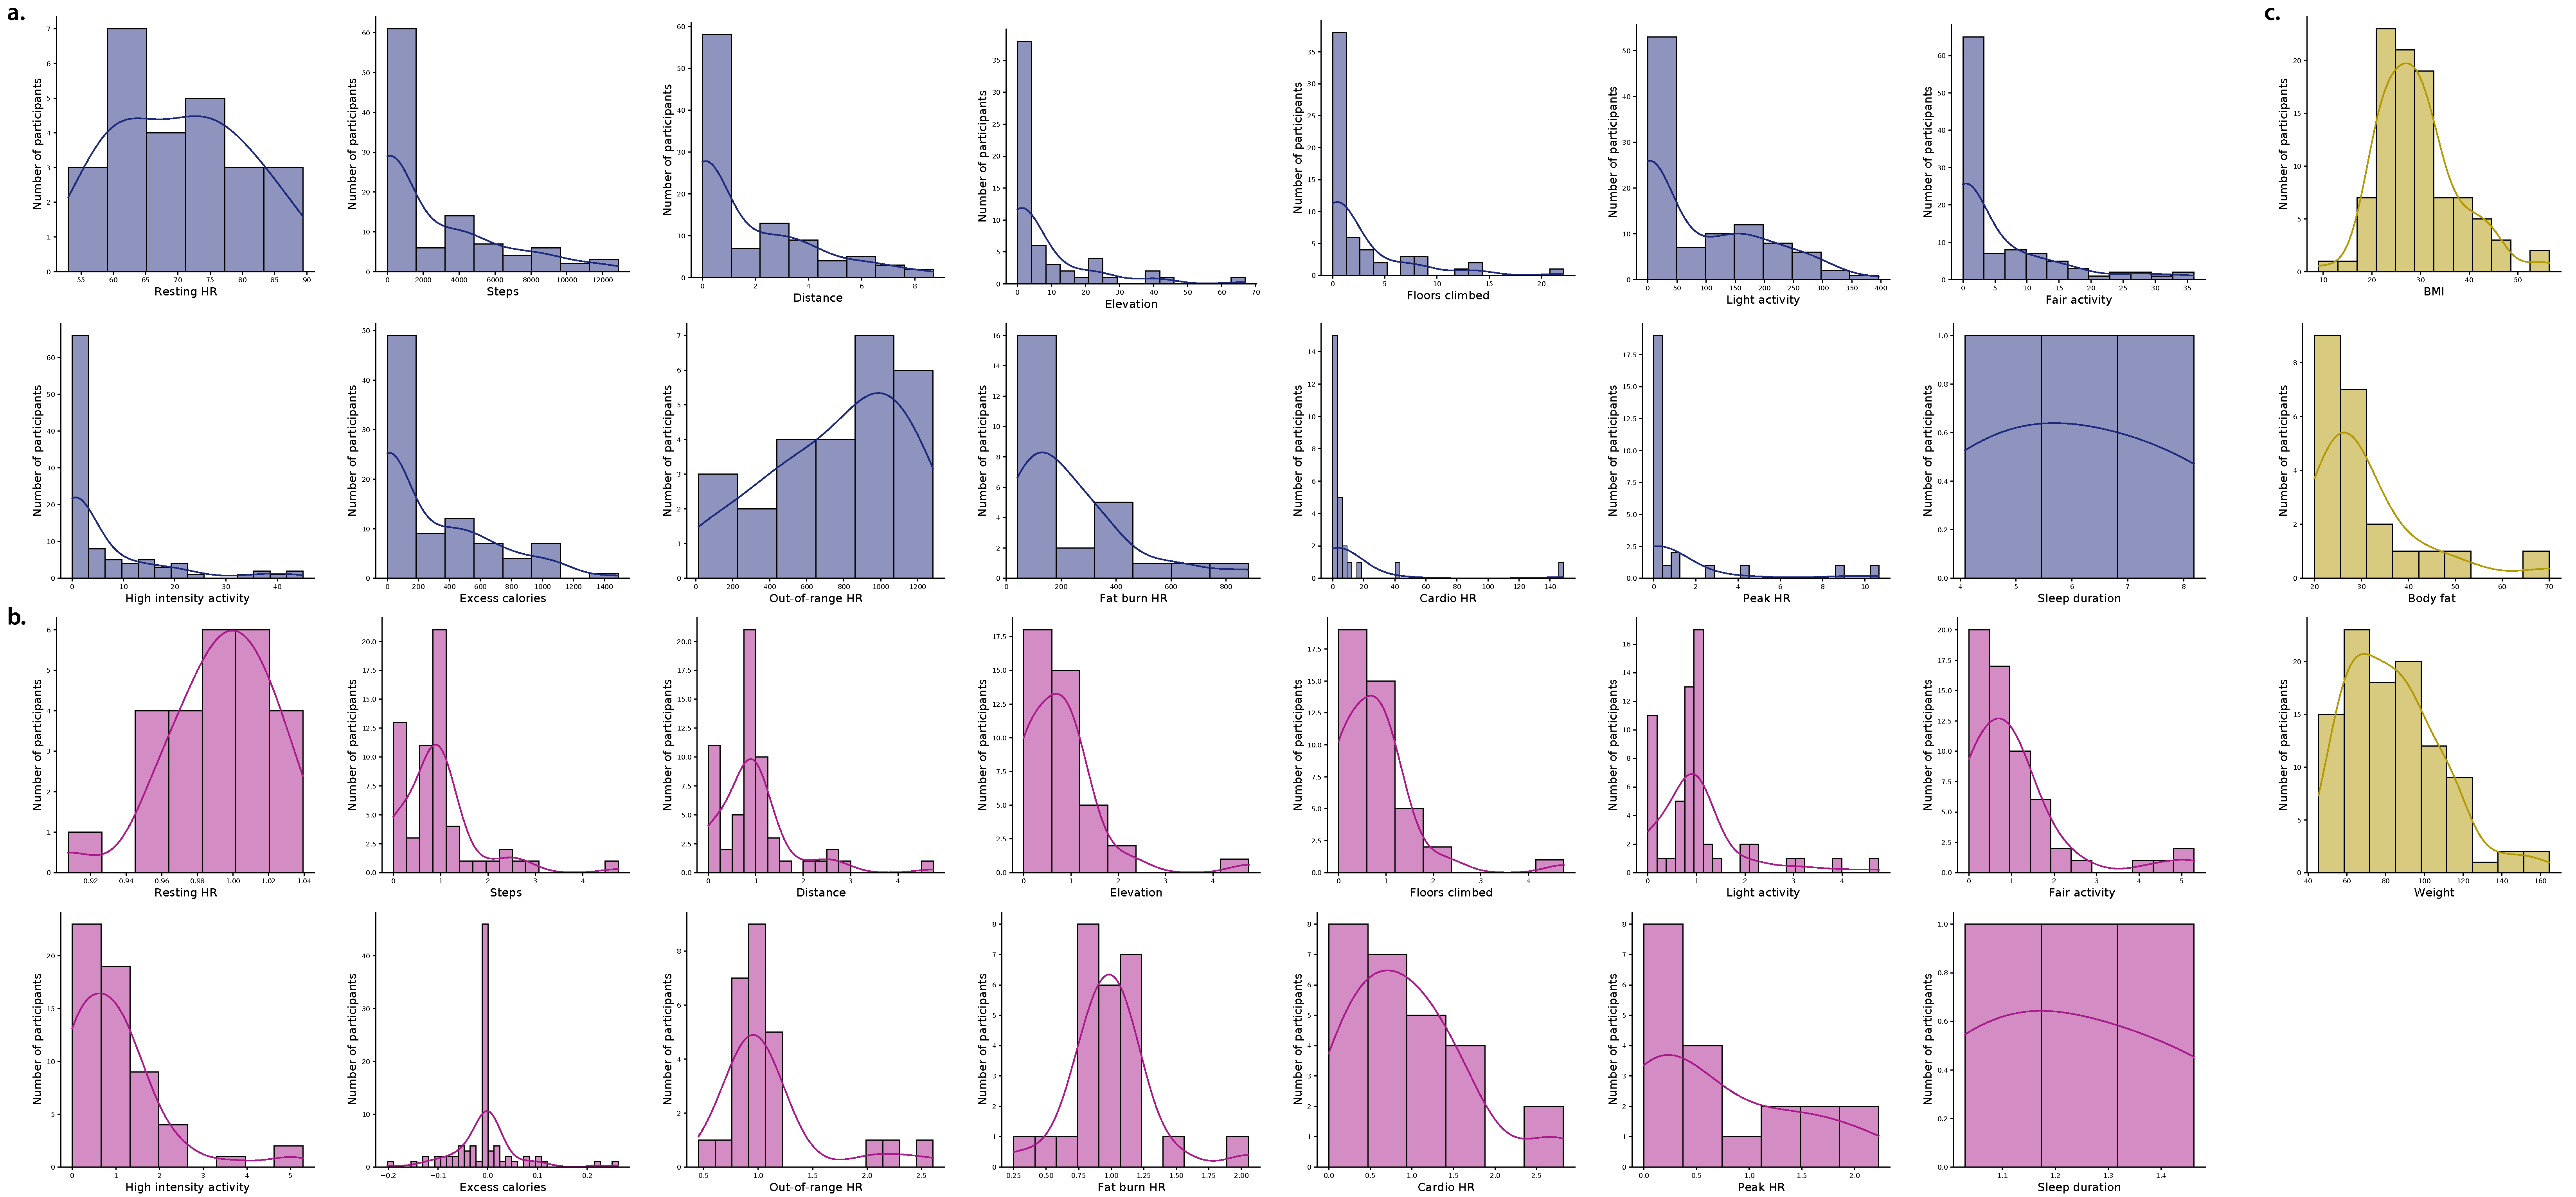
\includegraphics[width=\textwidth]{figs/fitness_distributions}
\caption{\textbf{Distributions of fitness measures.}}
\label{fig:fitness_dists}
\end{sidewaysfigure}

\begin{sidewaysfigure}[p]
\centering
\includegraphics[width=\textwidth]{figs/fitness_dists_immediate}
\caption{\textbf{Distributions of fitness measures, broken down
    by immediate task performance.}}
\label{fig:fitness_dists_immediate}
\end{sidewaysfigure}

\begin{sidewaysfigure}[p]
\centering
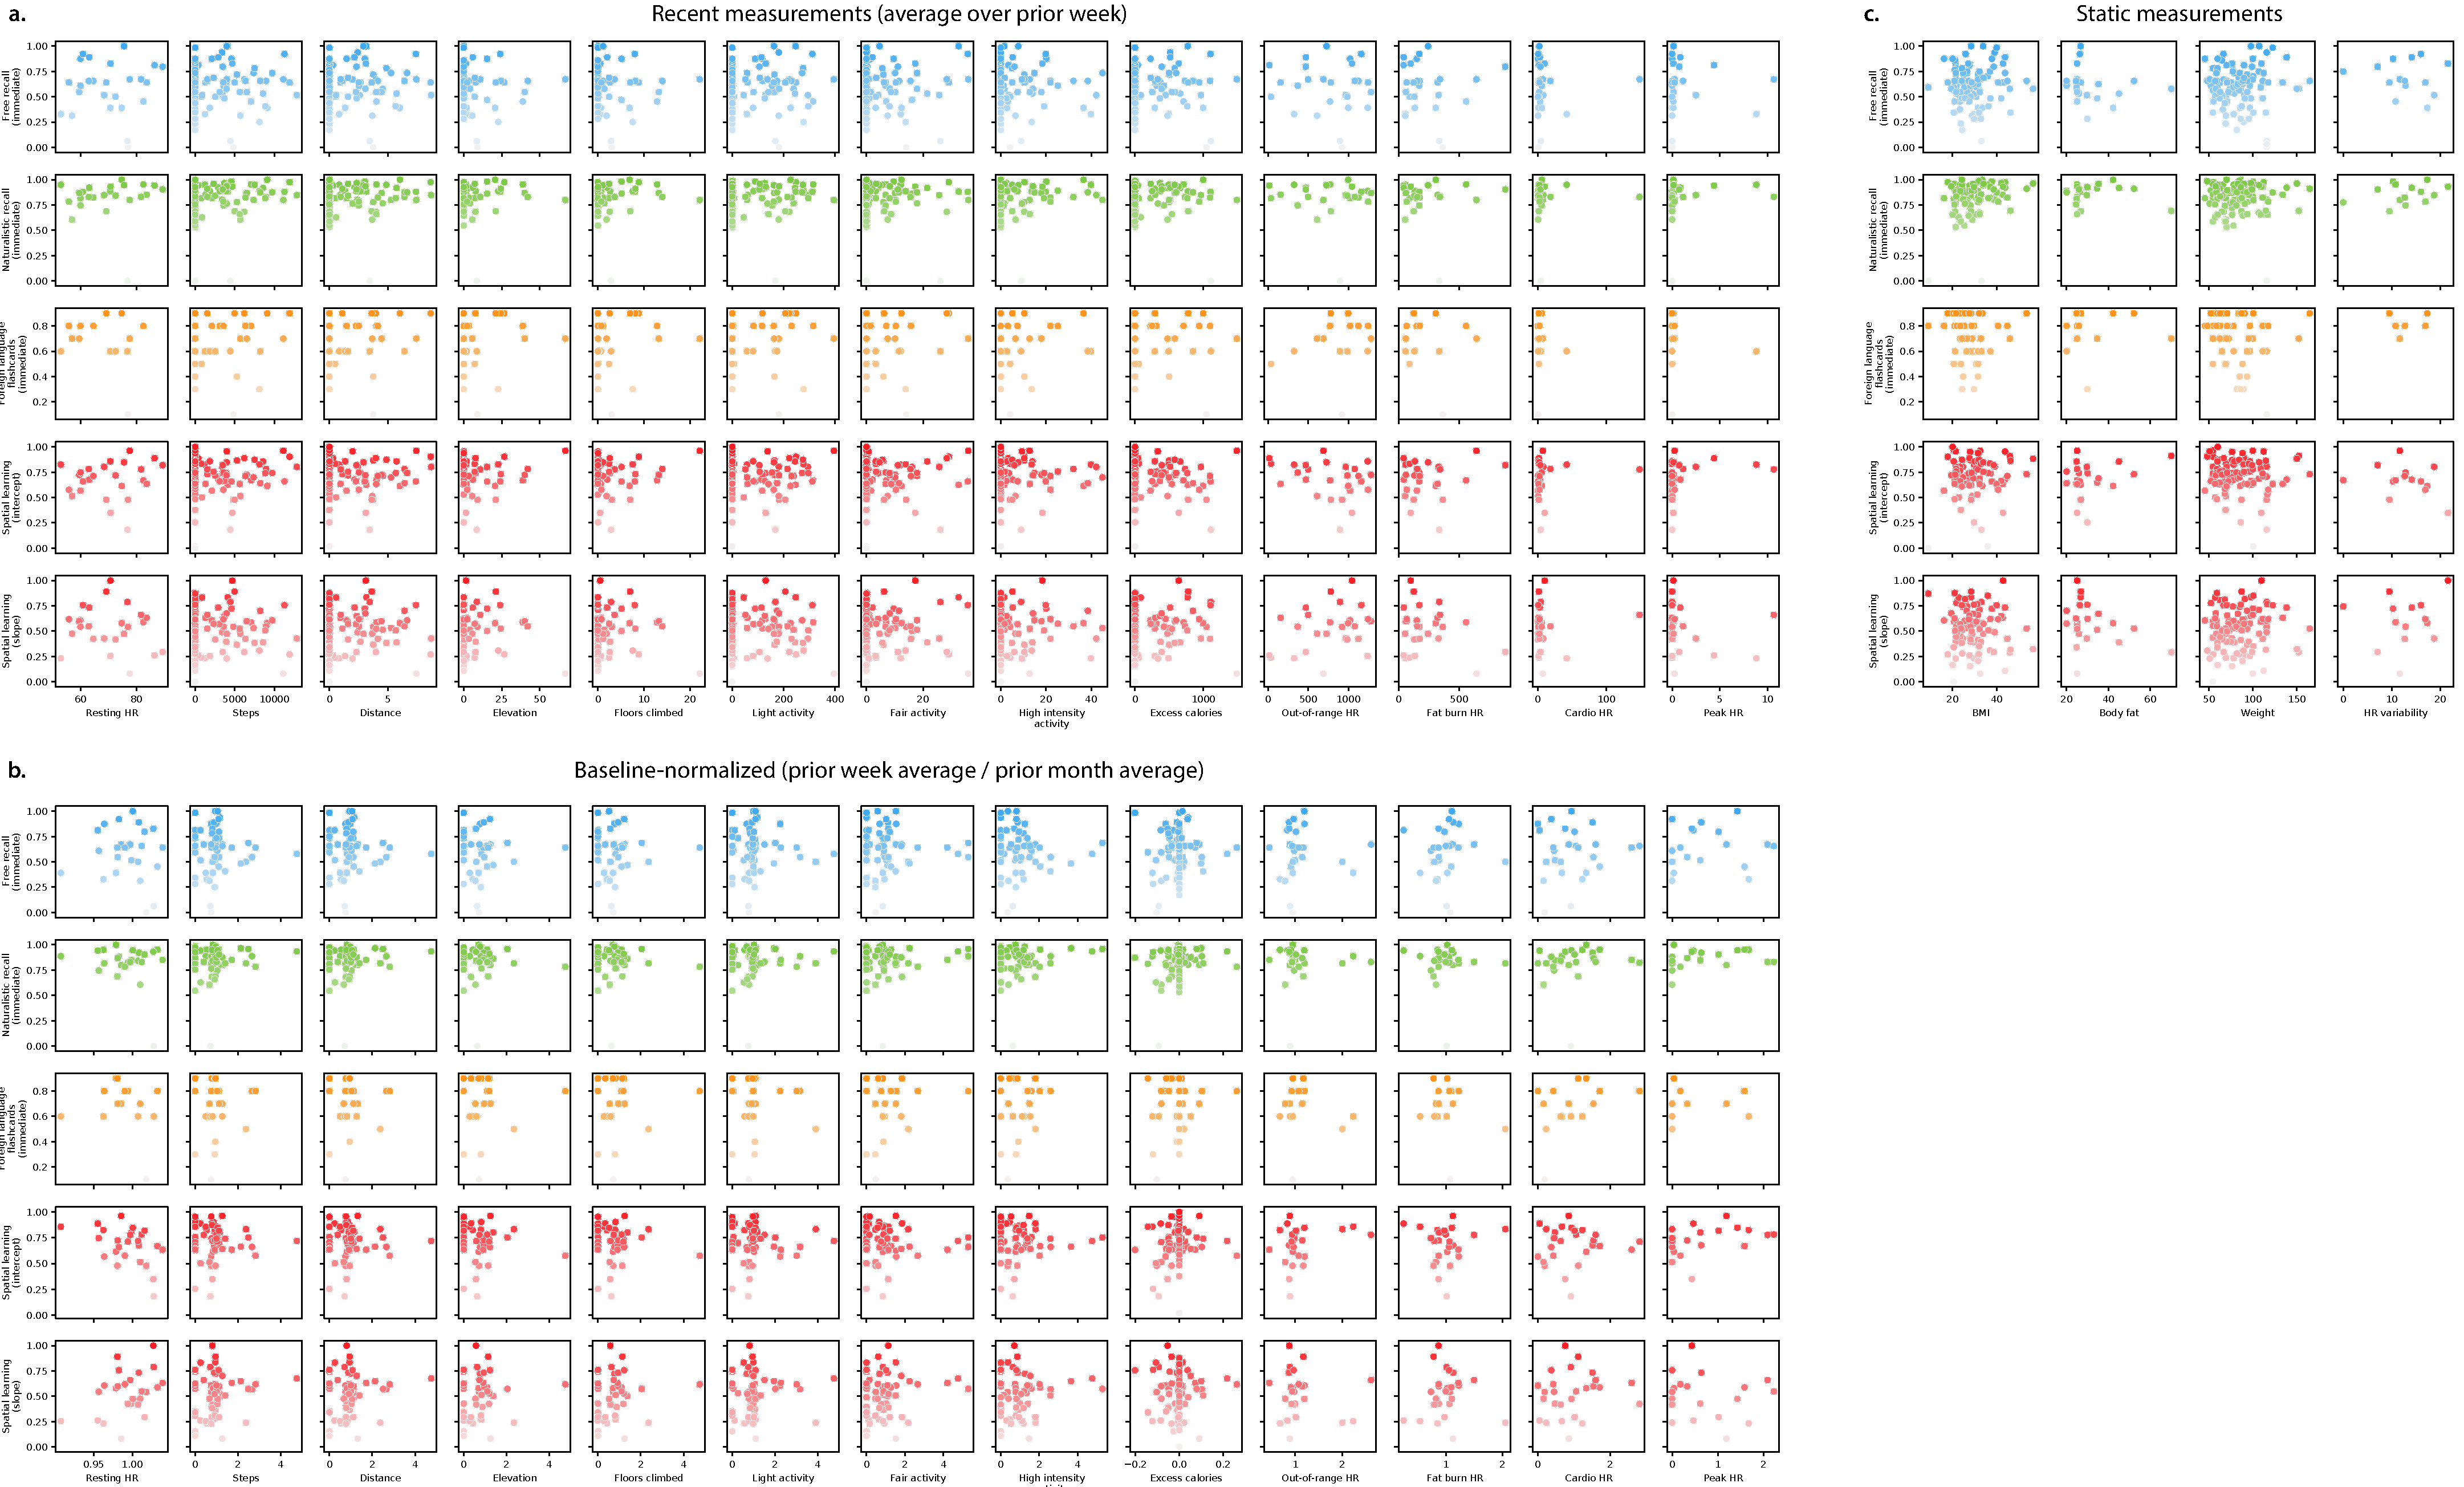
\includegraphics[width=\textwidth]{figs/fitness_scatter_immediate}
\caption{\textbf{Scatterplots of fitness measures versus
    immediate task performance measures.}}
\label{fig:fitness_scatters_immediate}
\end{sidewaysfigure}

\begin{sidewaysfigure}[p]
\centering
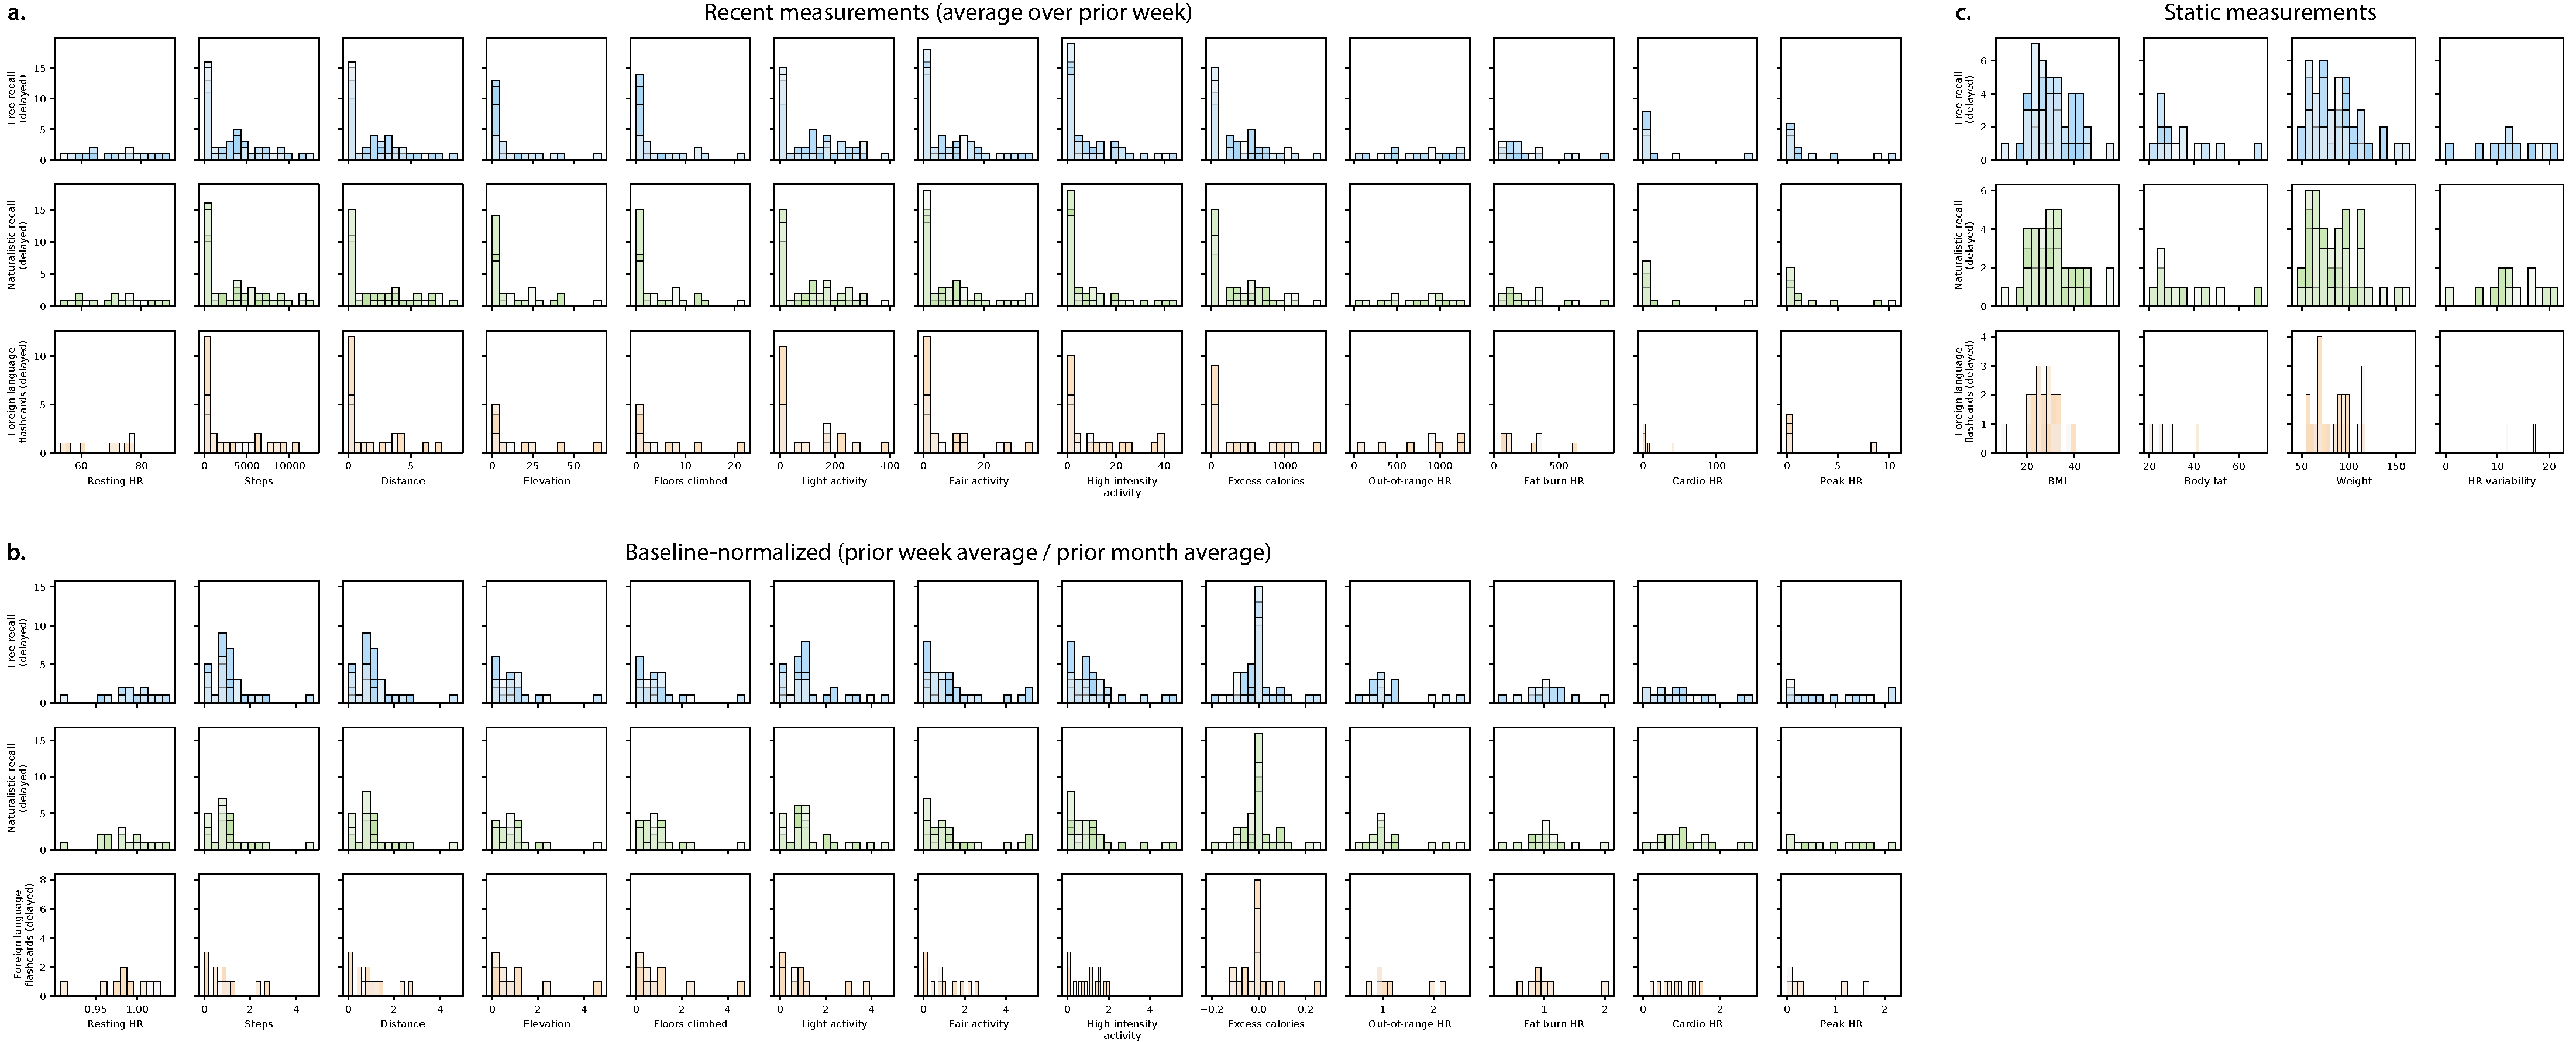
\includegraphics[width=\textwidth]{figs/fitness_dists_delayed}
\caption{\textbf{Distributions of fitness measures, broken down
    by delayed task performance.}}
\label{fig:fitness_dists_delayed}
\end{sidewaysfigure}

\begin{sidewaysfigure}[p]
\centering
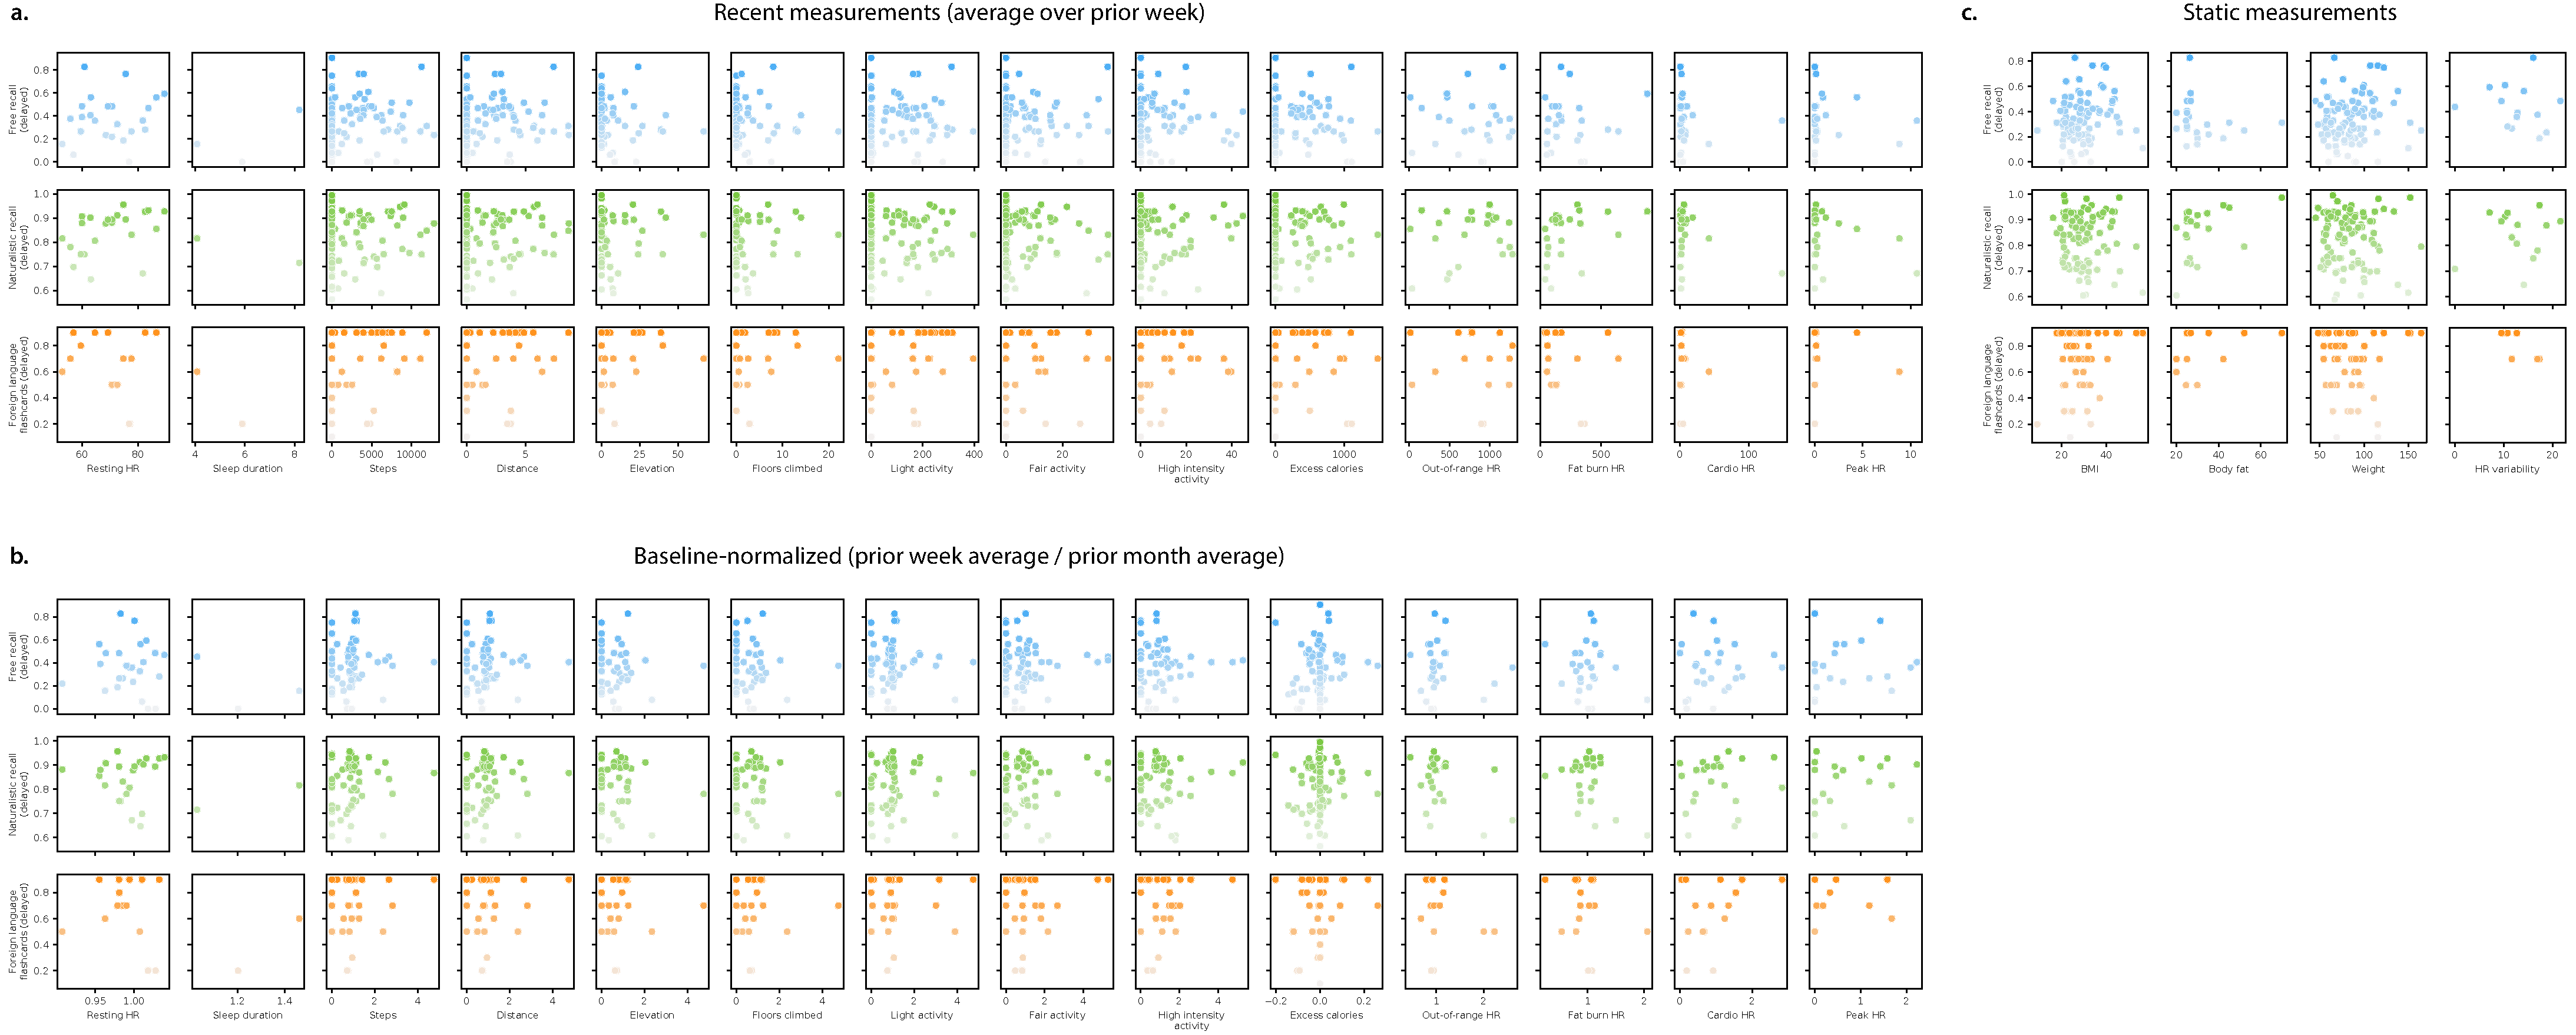
\includegraphics[width=\textwidth]{figs/fitness_scatter_delayed}
\caption{\textbf{Scatterplots of fitness measures versus
    delayed task performance measures.}}
\label{fig:fitness_scatters_delayed}
\end{sidewaysfigure}

\begin{figure}[p]
\centering
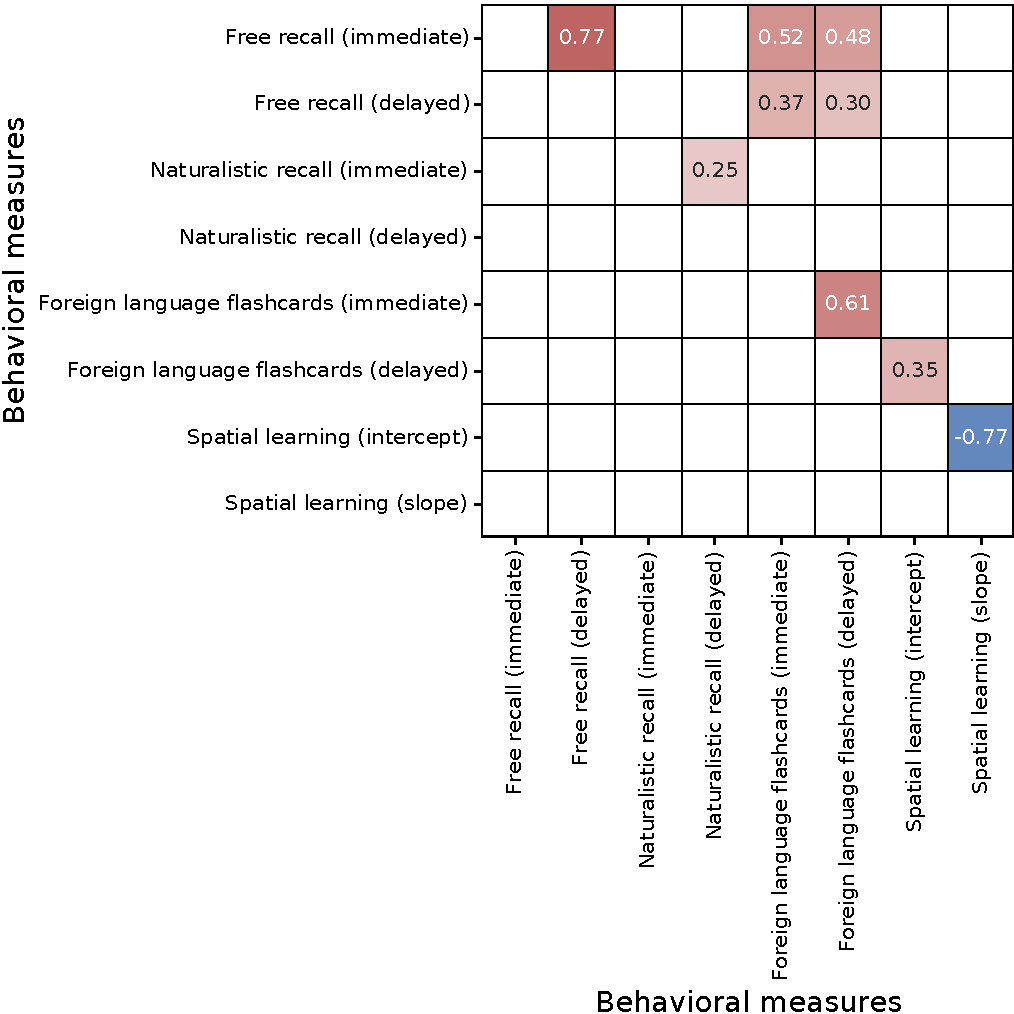
\includegraphics[width=0.4\textwidth]{figs/behavior_behavior_correlations}
\caption{\textbf{Bootstrap-estimated reliable correlations between
    behavioral measures.}}
\label{fig:behavioral_corrs}
\end{figure}

\begin{figure}[p]
\centering
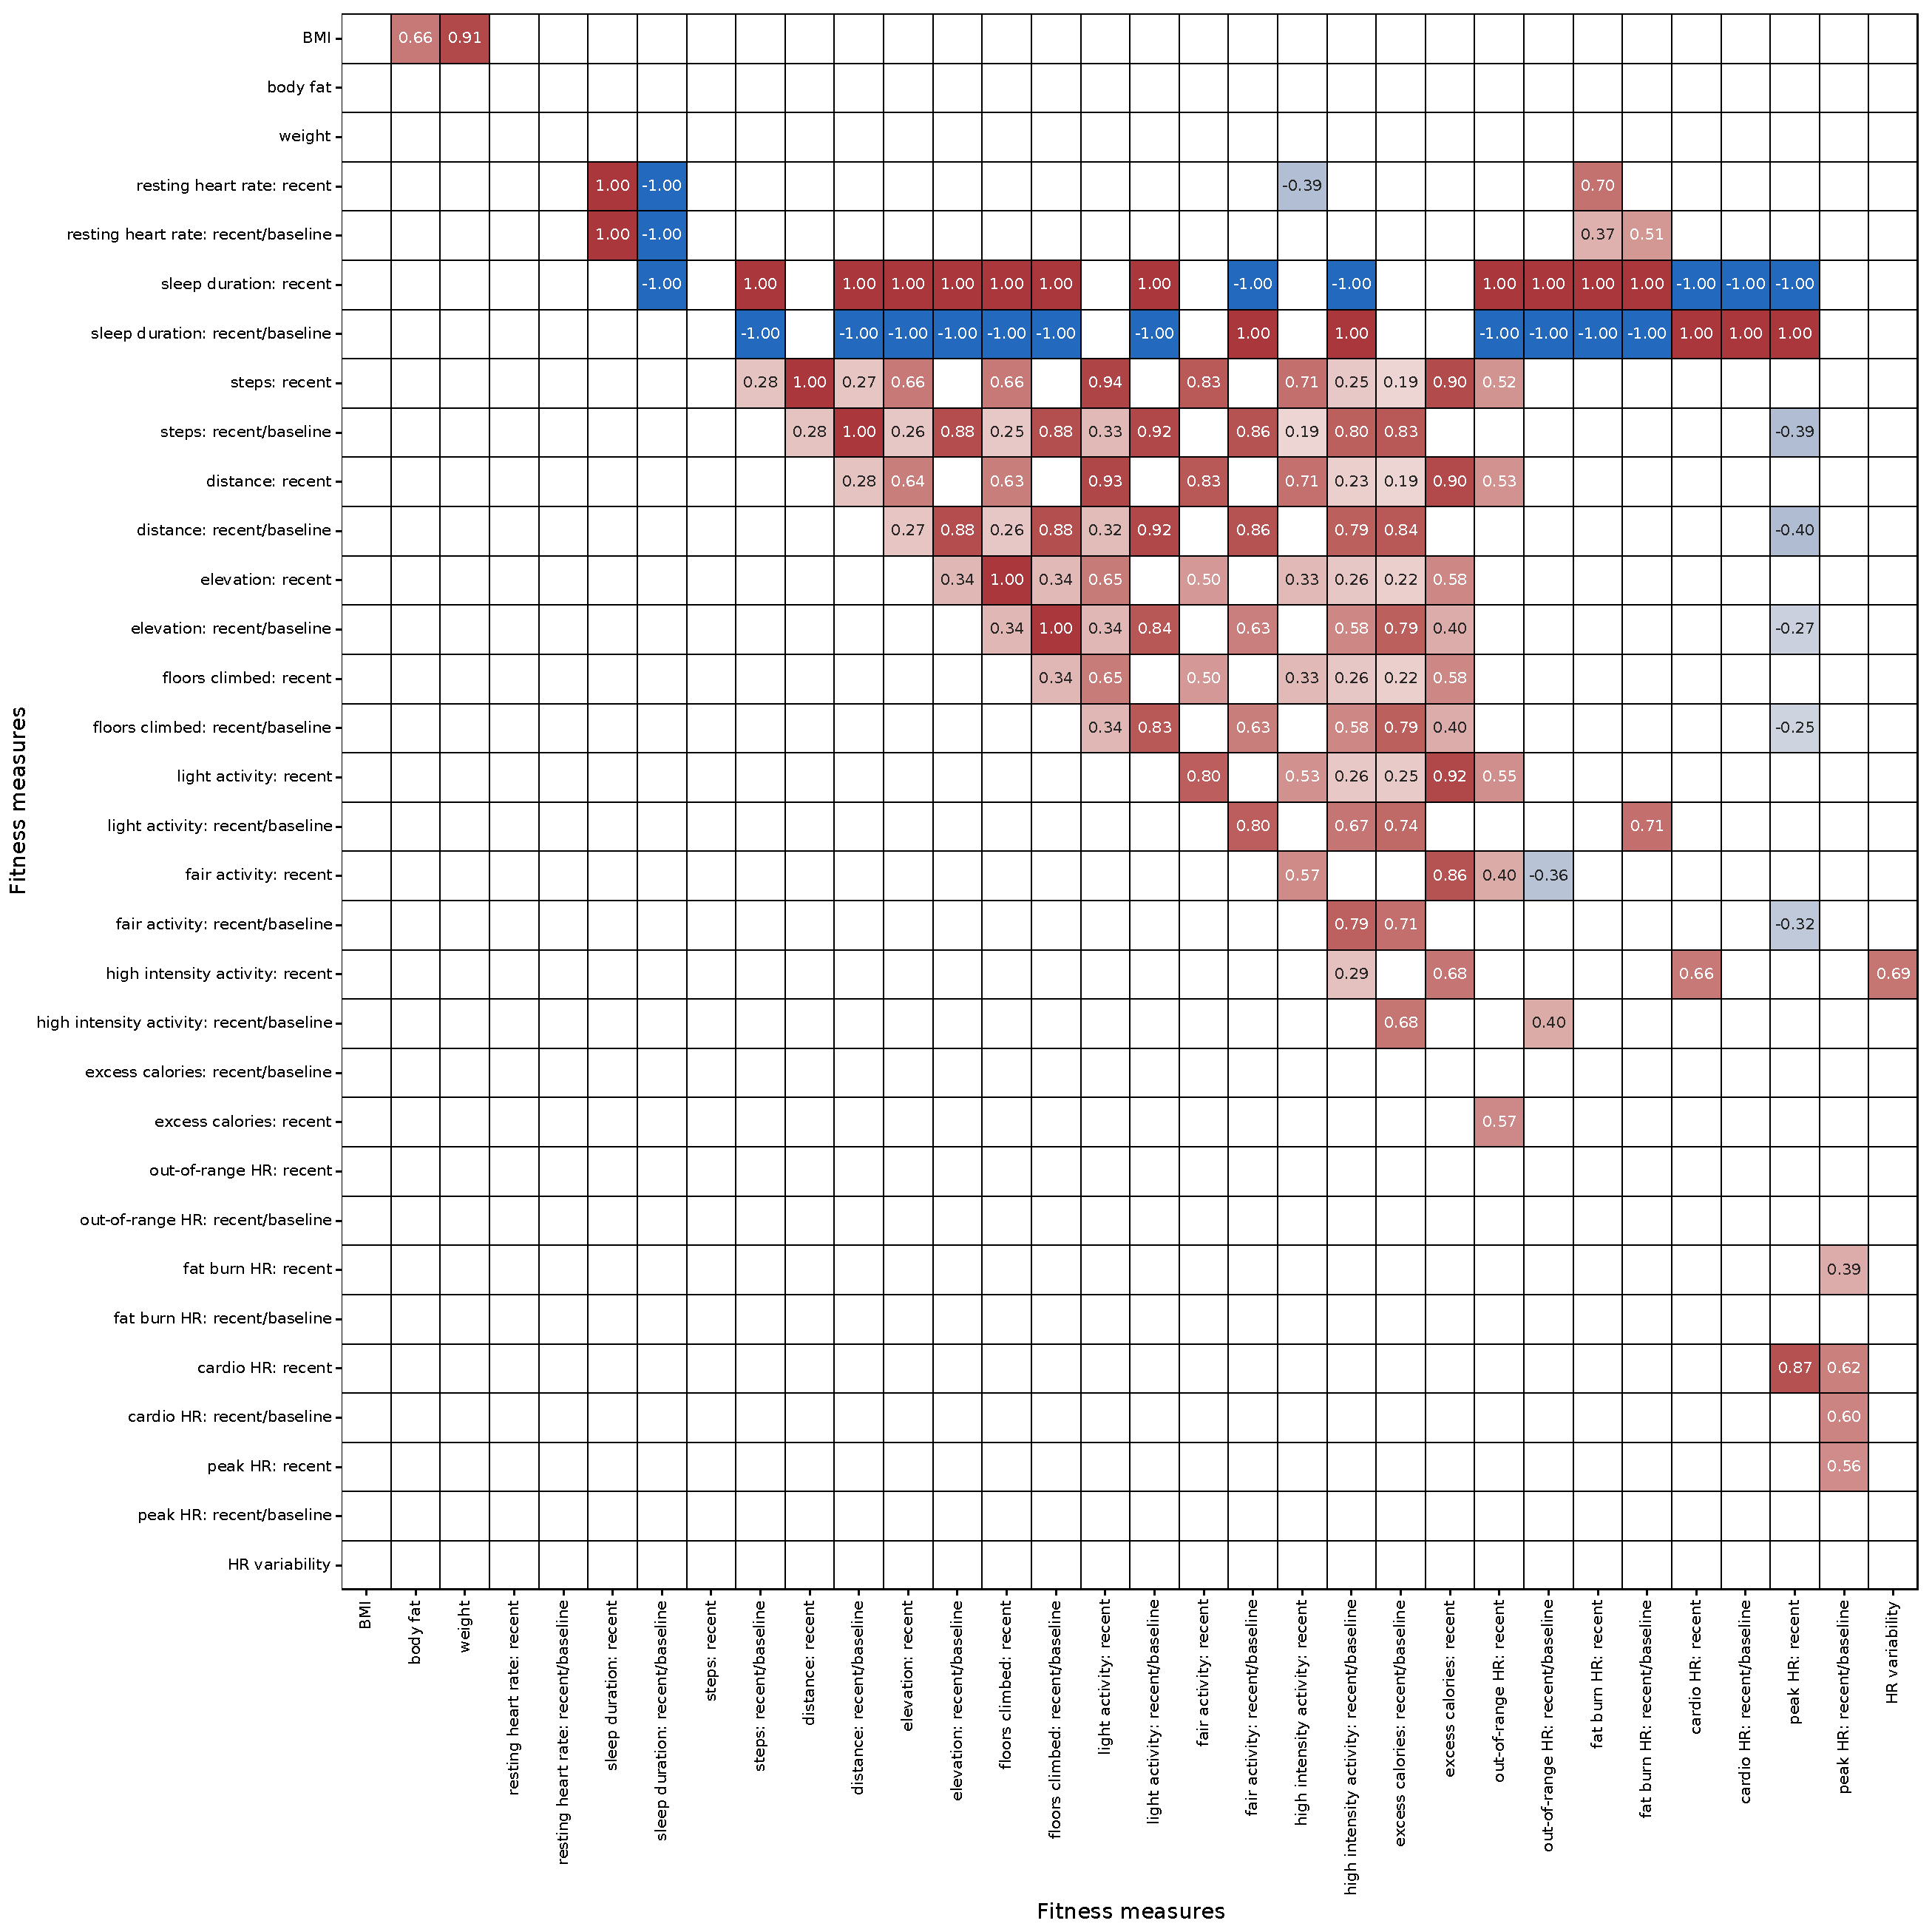
\includegraphics[width=\textwidth]{figs/fitness_fitness_correlations}
\caption{\textbf{Bootstrap-estimated reliable correlations between
    fitness measures.}}
\label{fig:fitness_corrs}
\end{figure}

\begin{figure}[p]
\centering
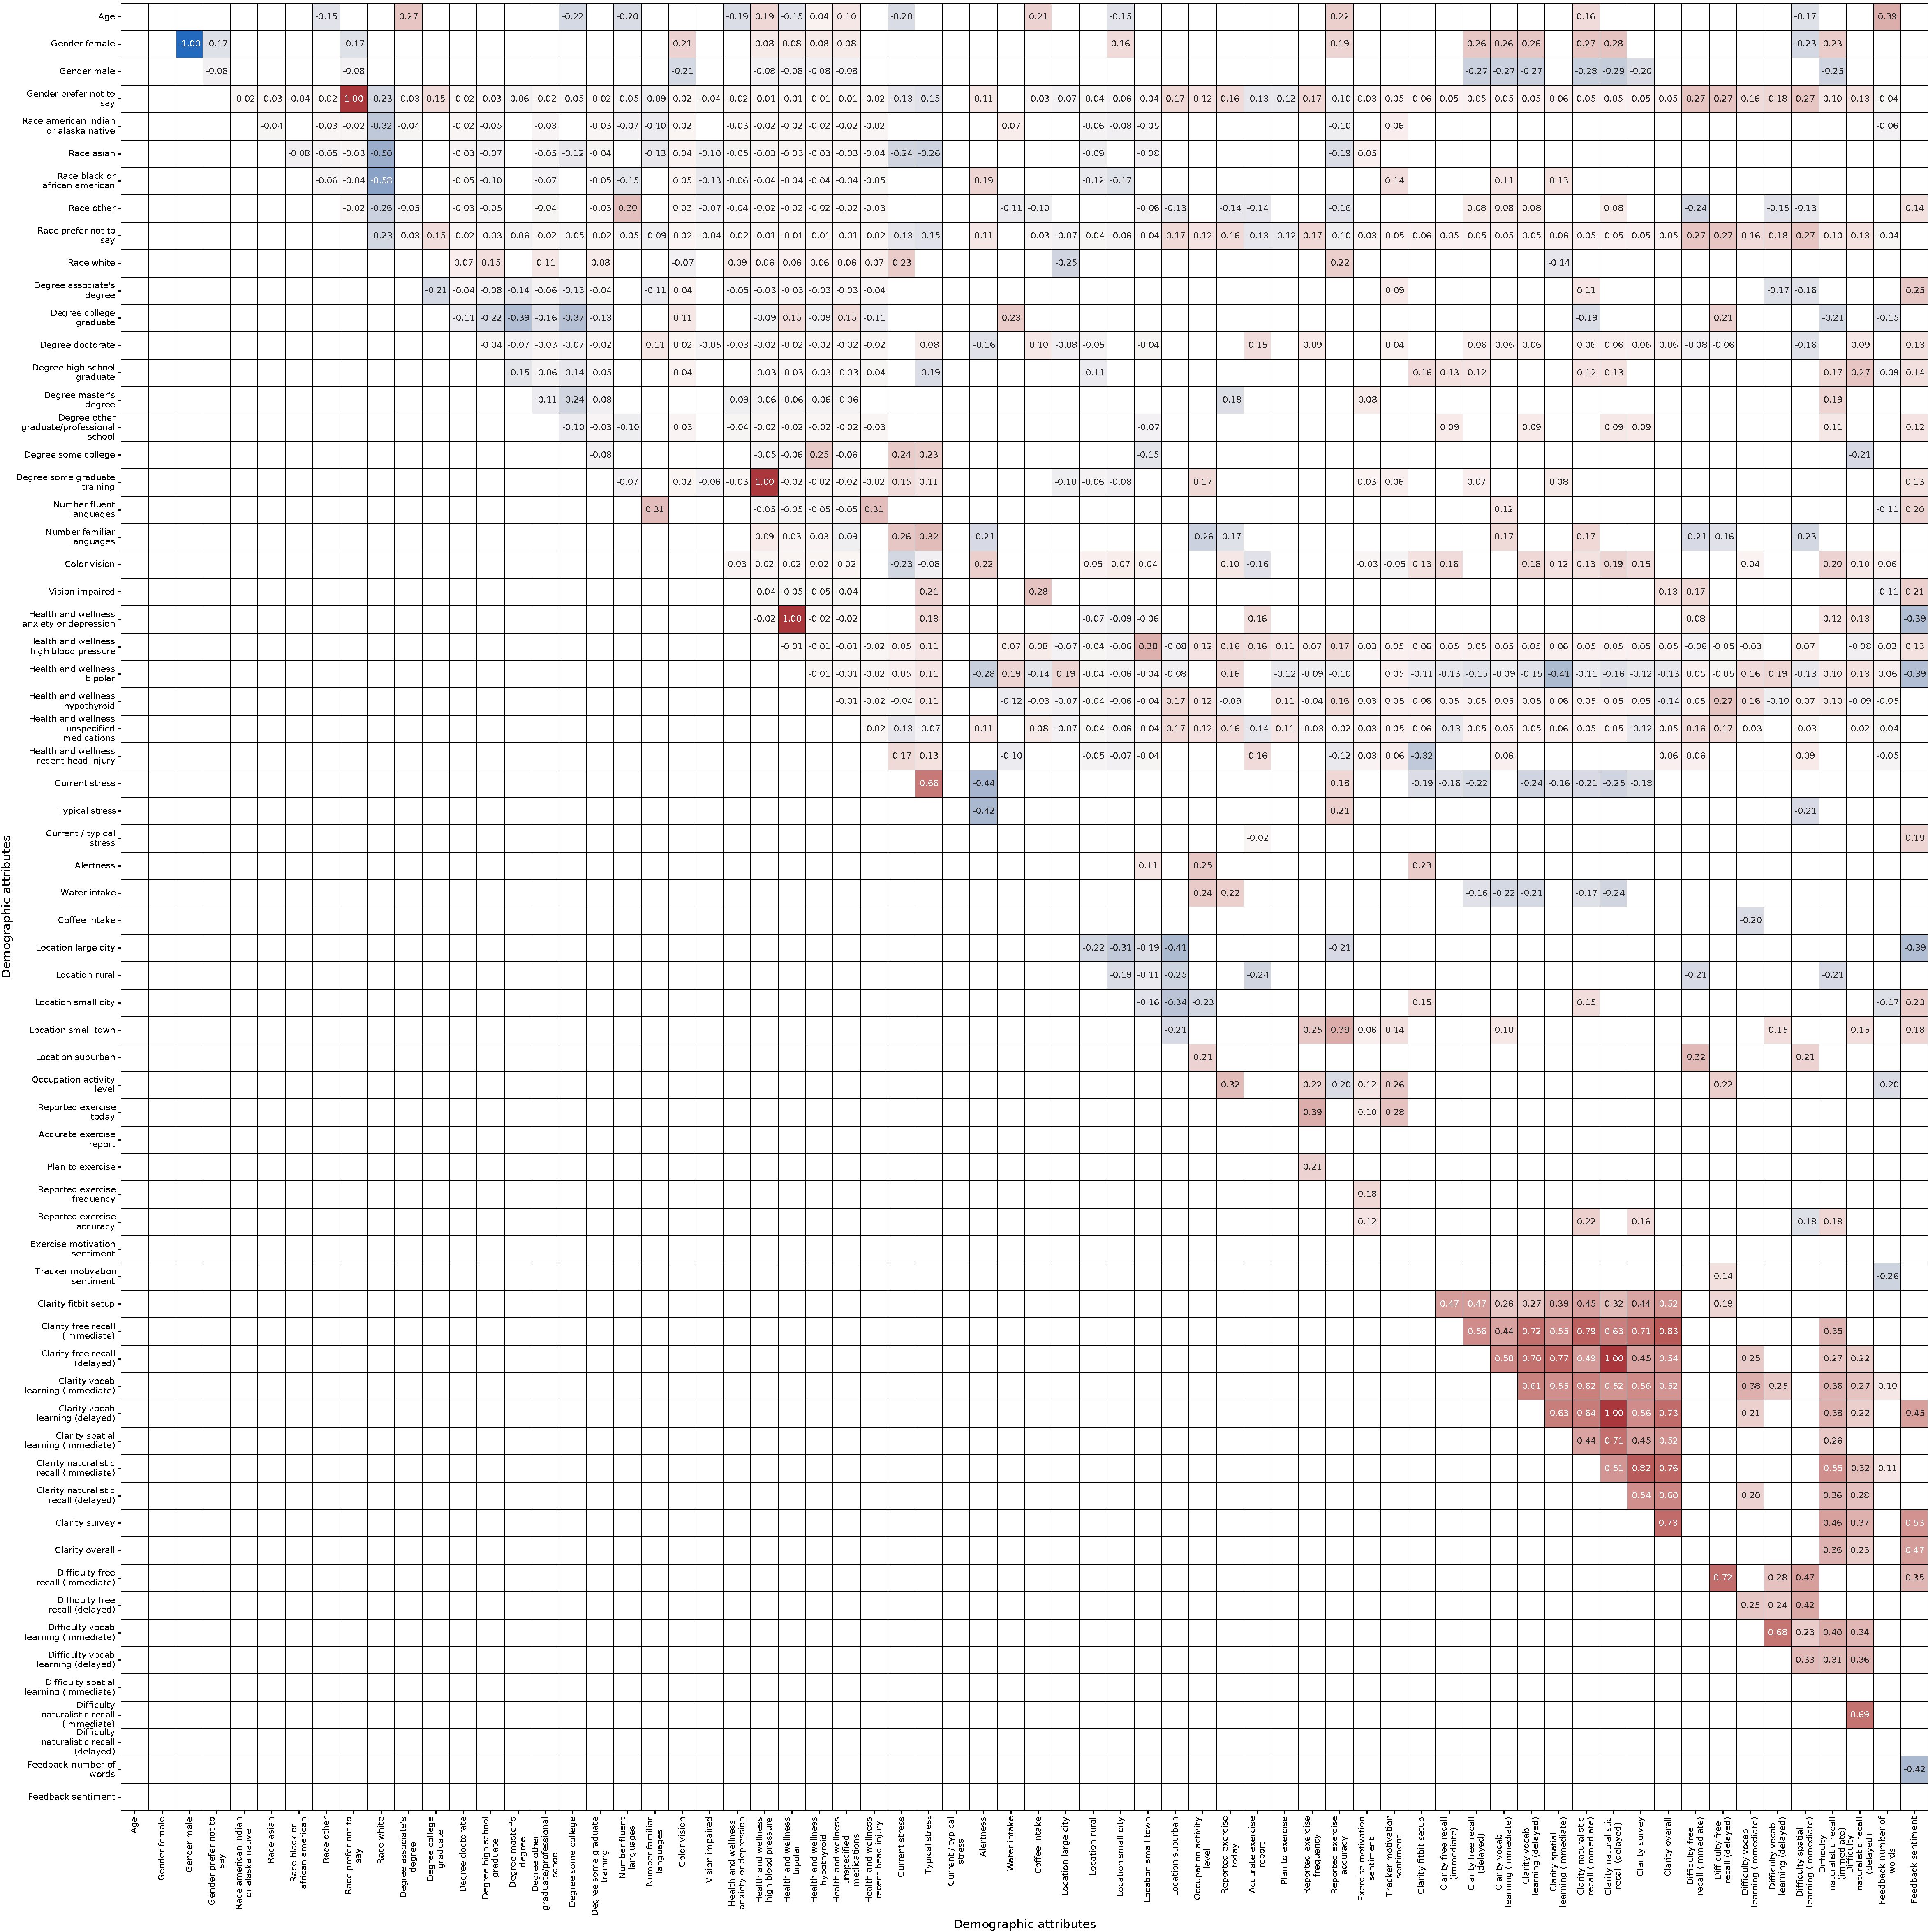
\includegraphics[width=\textwidth]{figs/survey_survey_correlations}
\caption{\textbf{Bootstrap-estimated reliable correlations between
    demographic measures.}}
\label{fig:survey_corrs}
\end{figure}

\begin{sidewaysfigure}[p]
\centering
\includegraphics[width=\textwidth]{figs/behavior_fitness+survey_correlations}
\caption{\textbf{Bootstrap-estimated reliable correlations between
    behavioral measures and fitness or demographic measures.}}
\label{fig:fitness_survey_corrs}
\end{sidewaysfigure}

\begin{figure}[p]
  \centering
  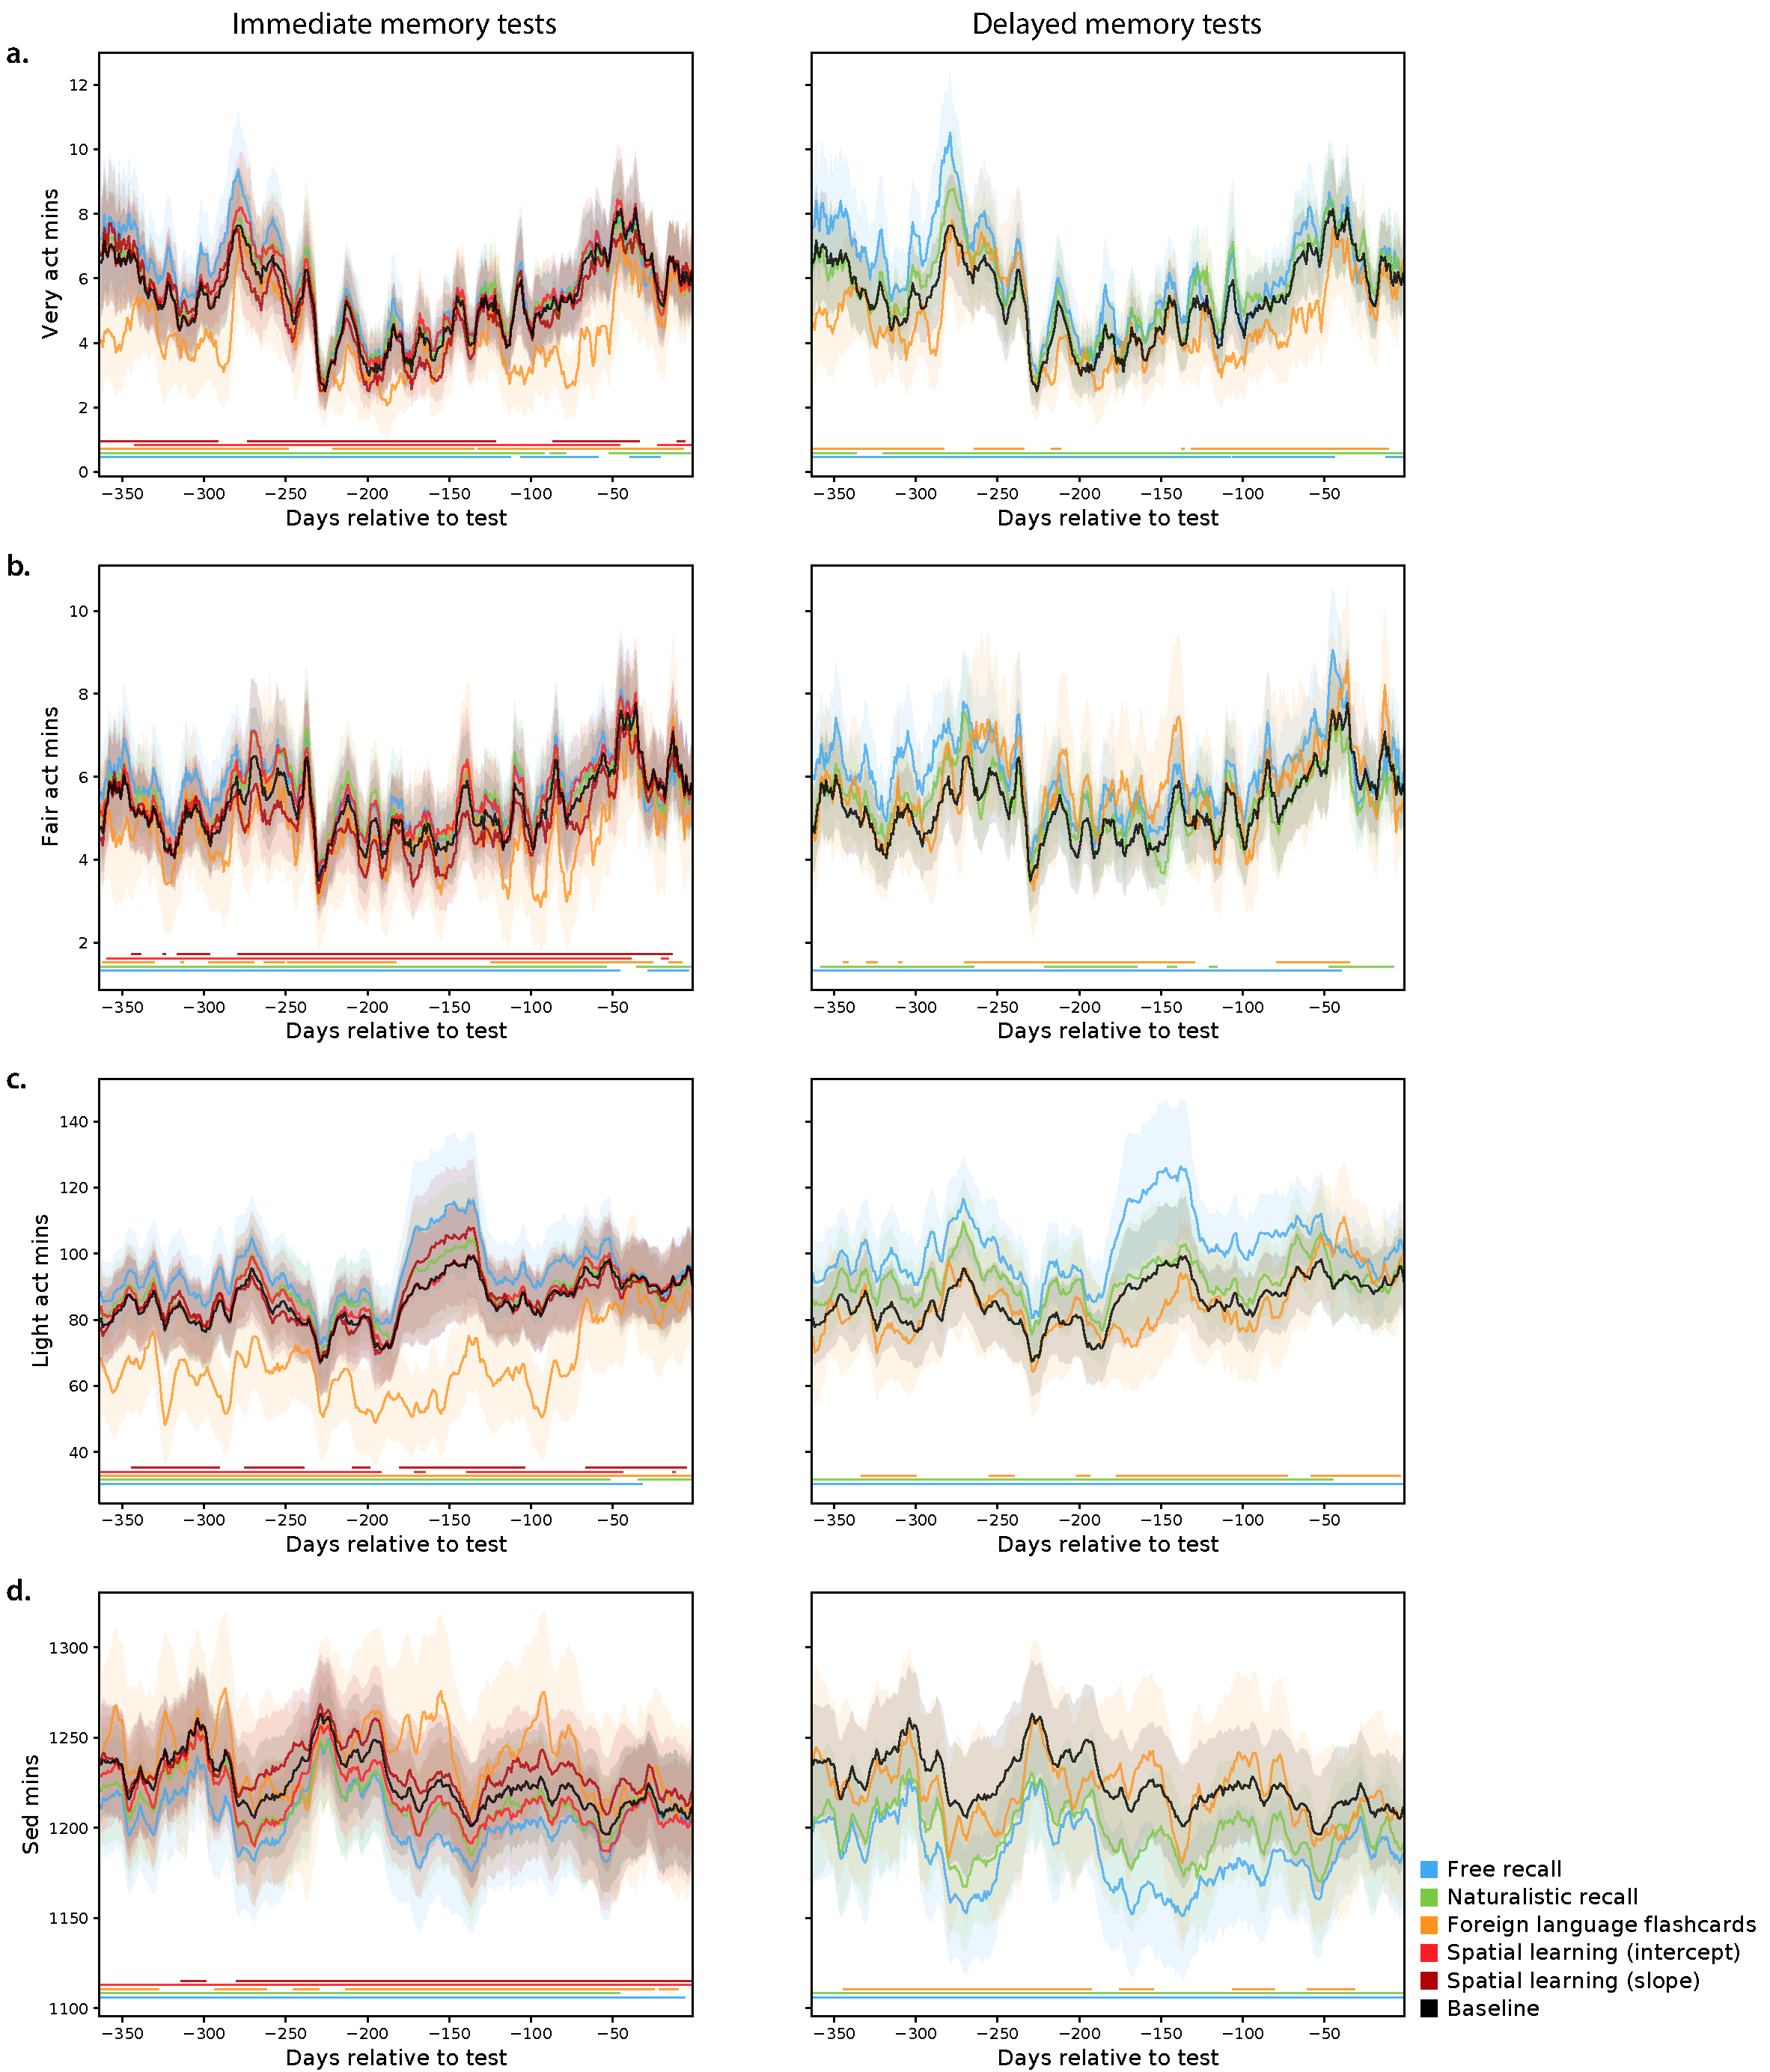
\includegraphics[width=0.75\textwidth]{figs/weighted_timecourse_activity}
\caption{\textbf{History of fitness activity levels weighted by
    behavioral performance.}}
\label{fig:activity_timecourse}
\end{figure}

\begin{figure}[p]
  \centering
  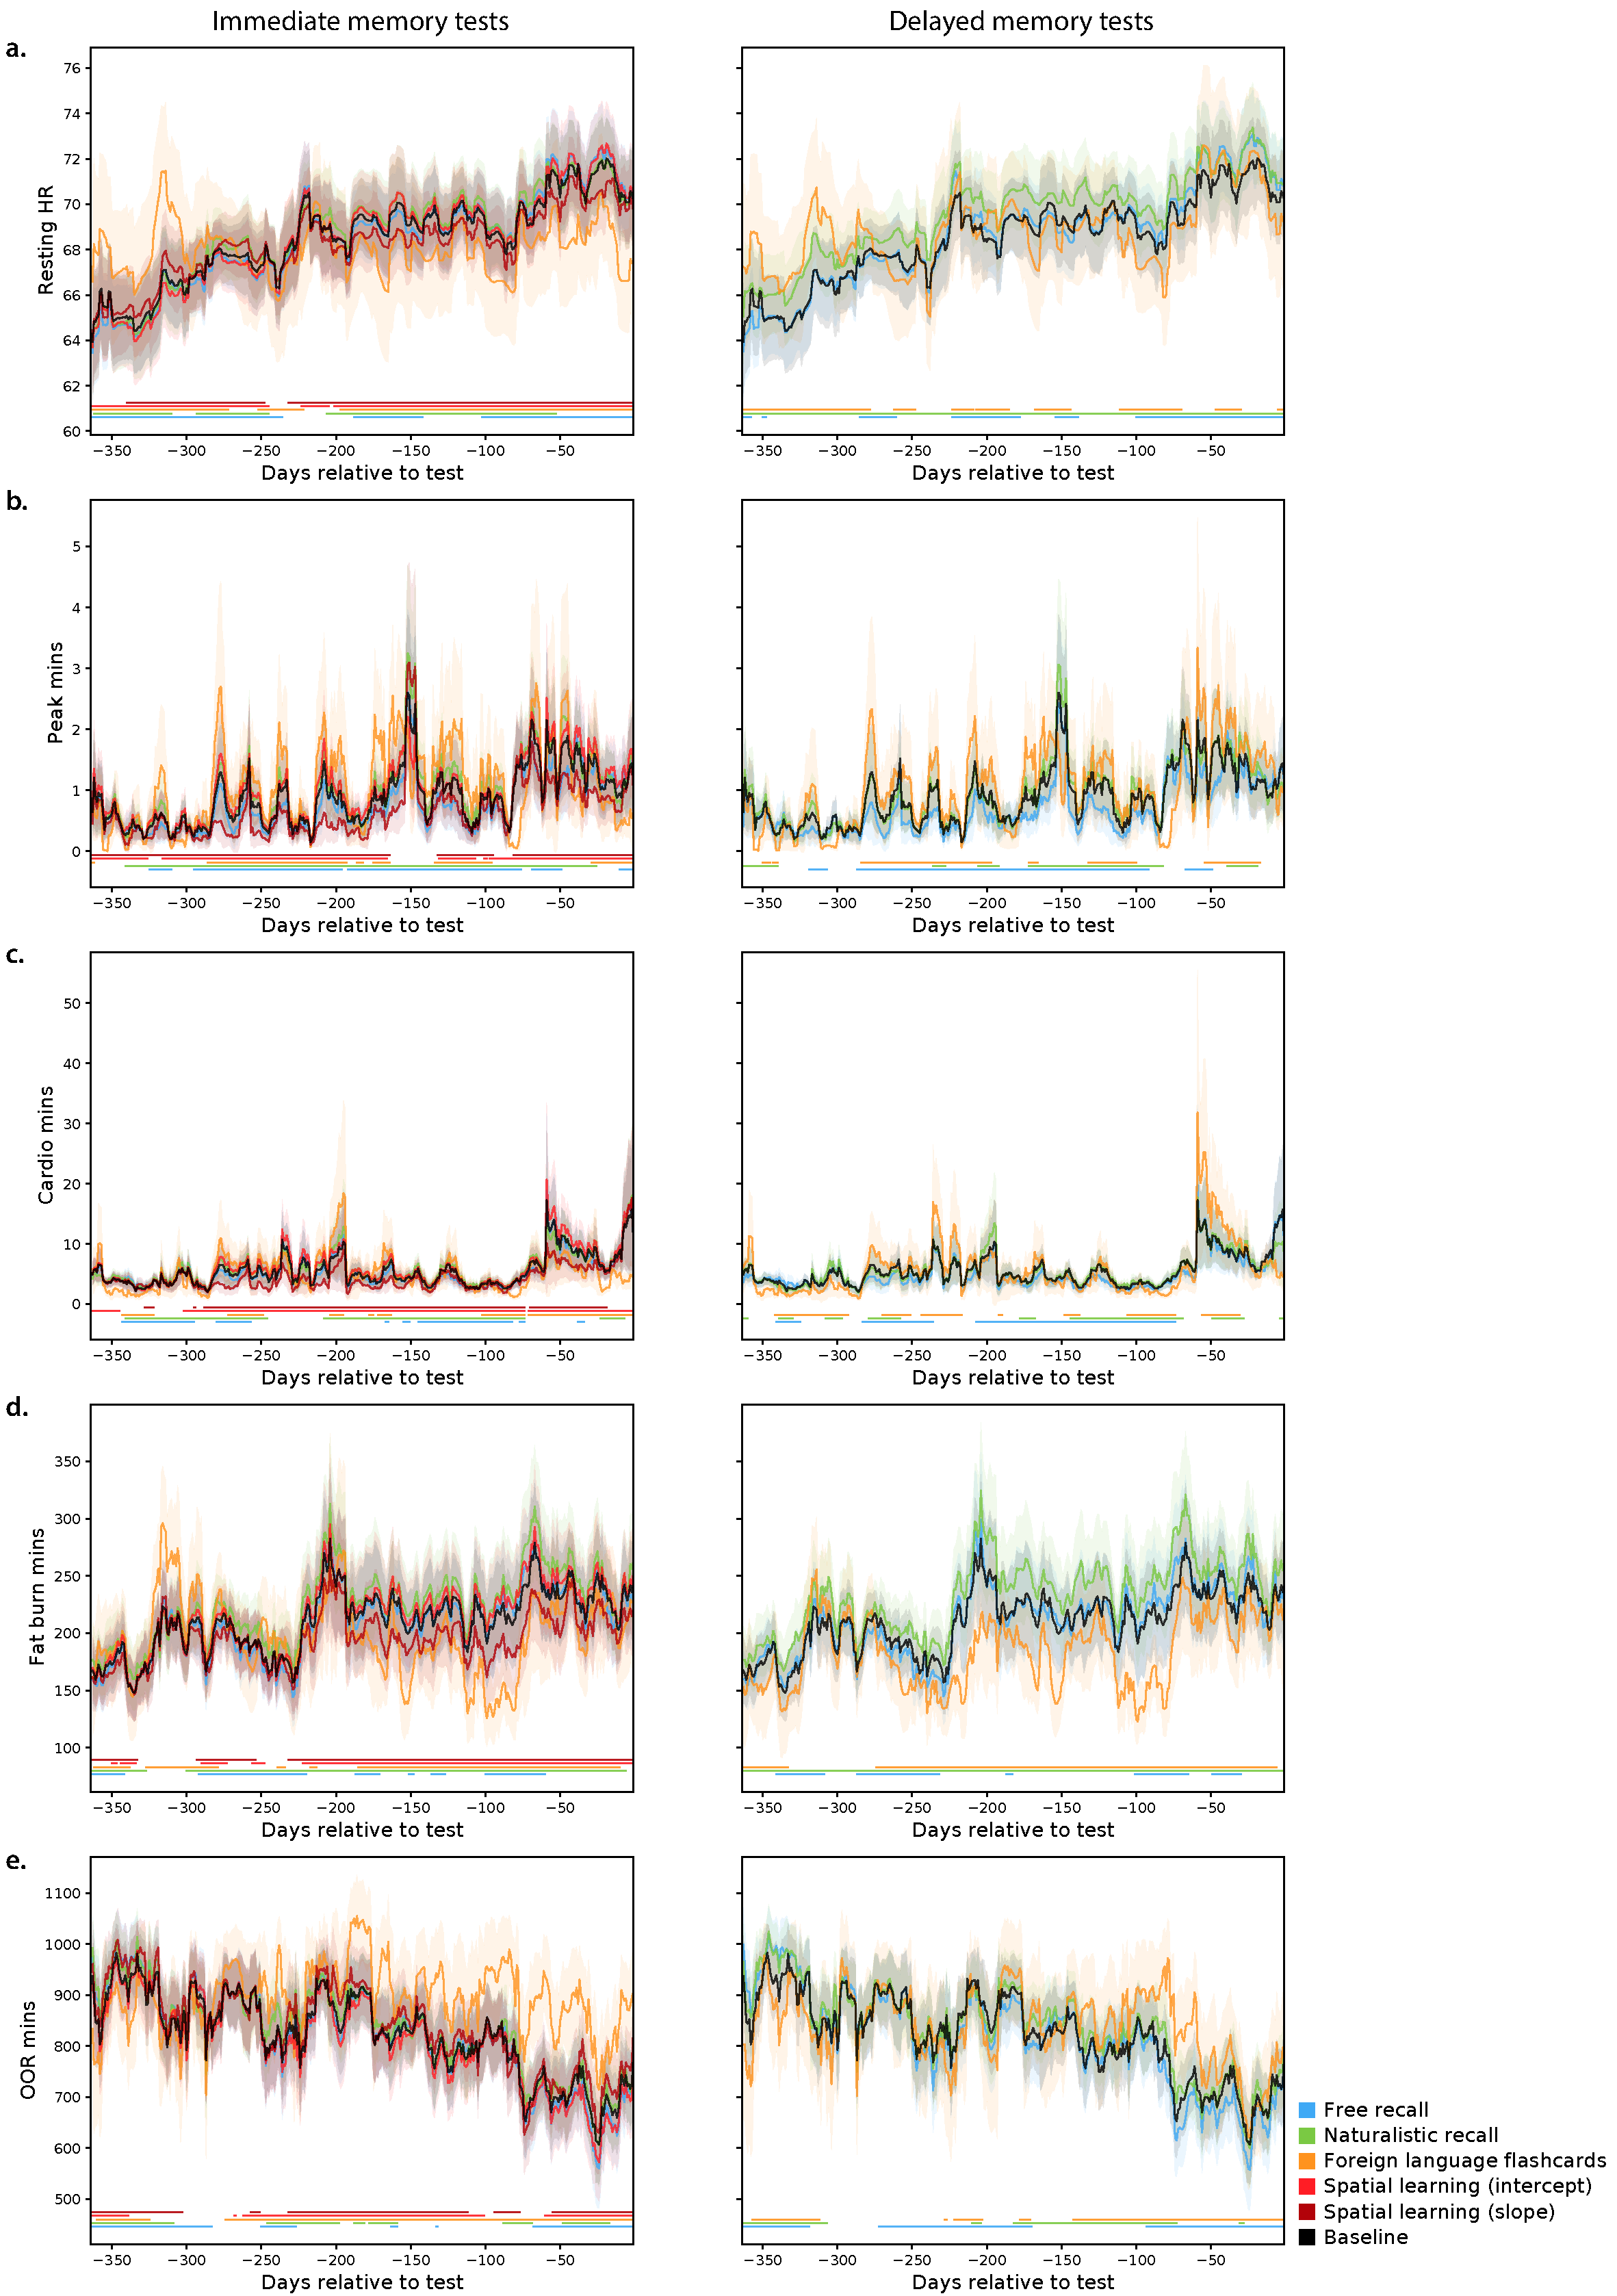
\includegraphics[width=0.7\textwidth]{figs/weighted_timecourse_HR}
\caption{\textbf{History of cardiovascular activity weighted by
    behavioral performance.}}
\label{fig:HR_timecourse}
  \end{figure}

\begin{figure}[p]
  \centering
  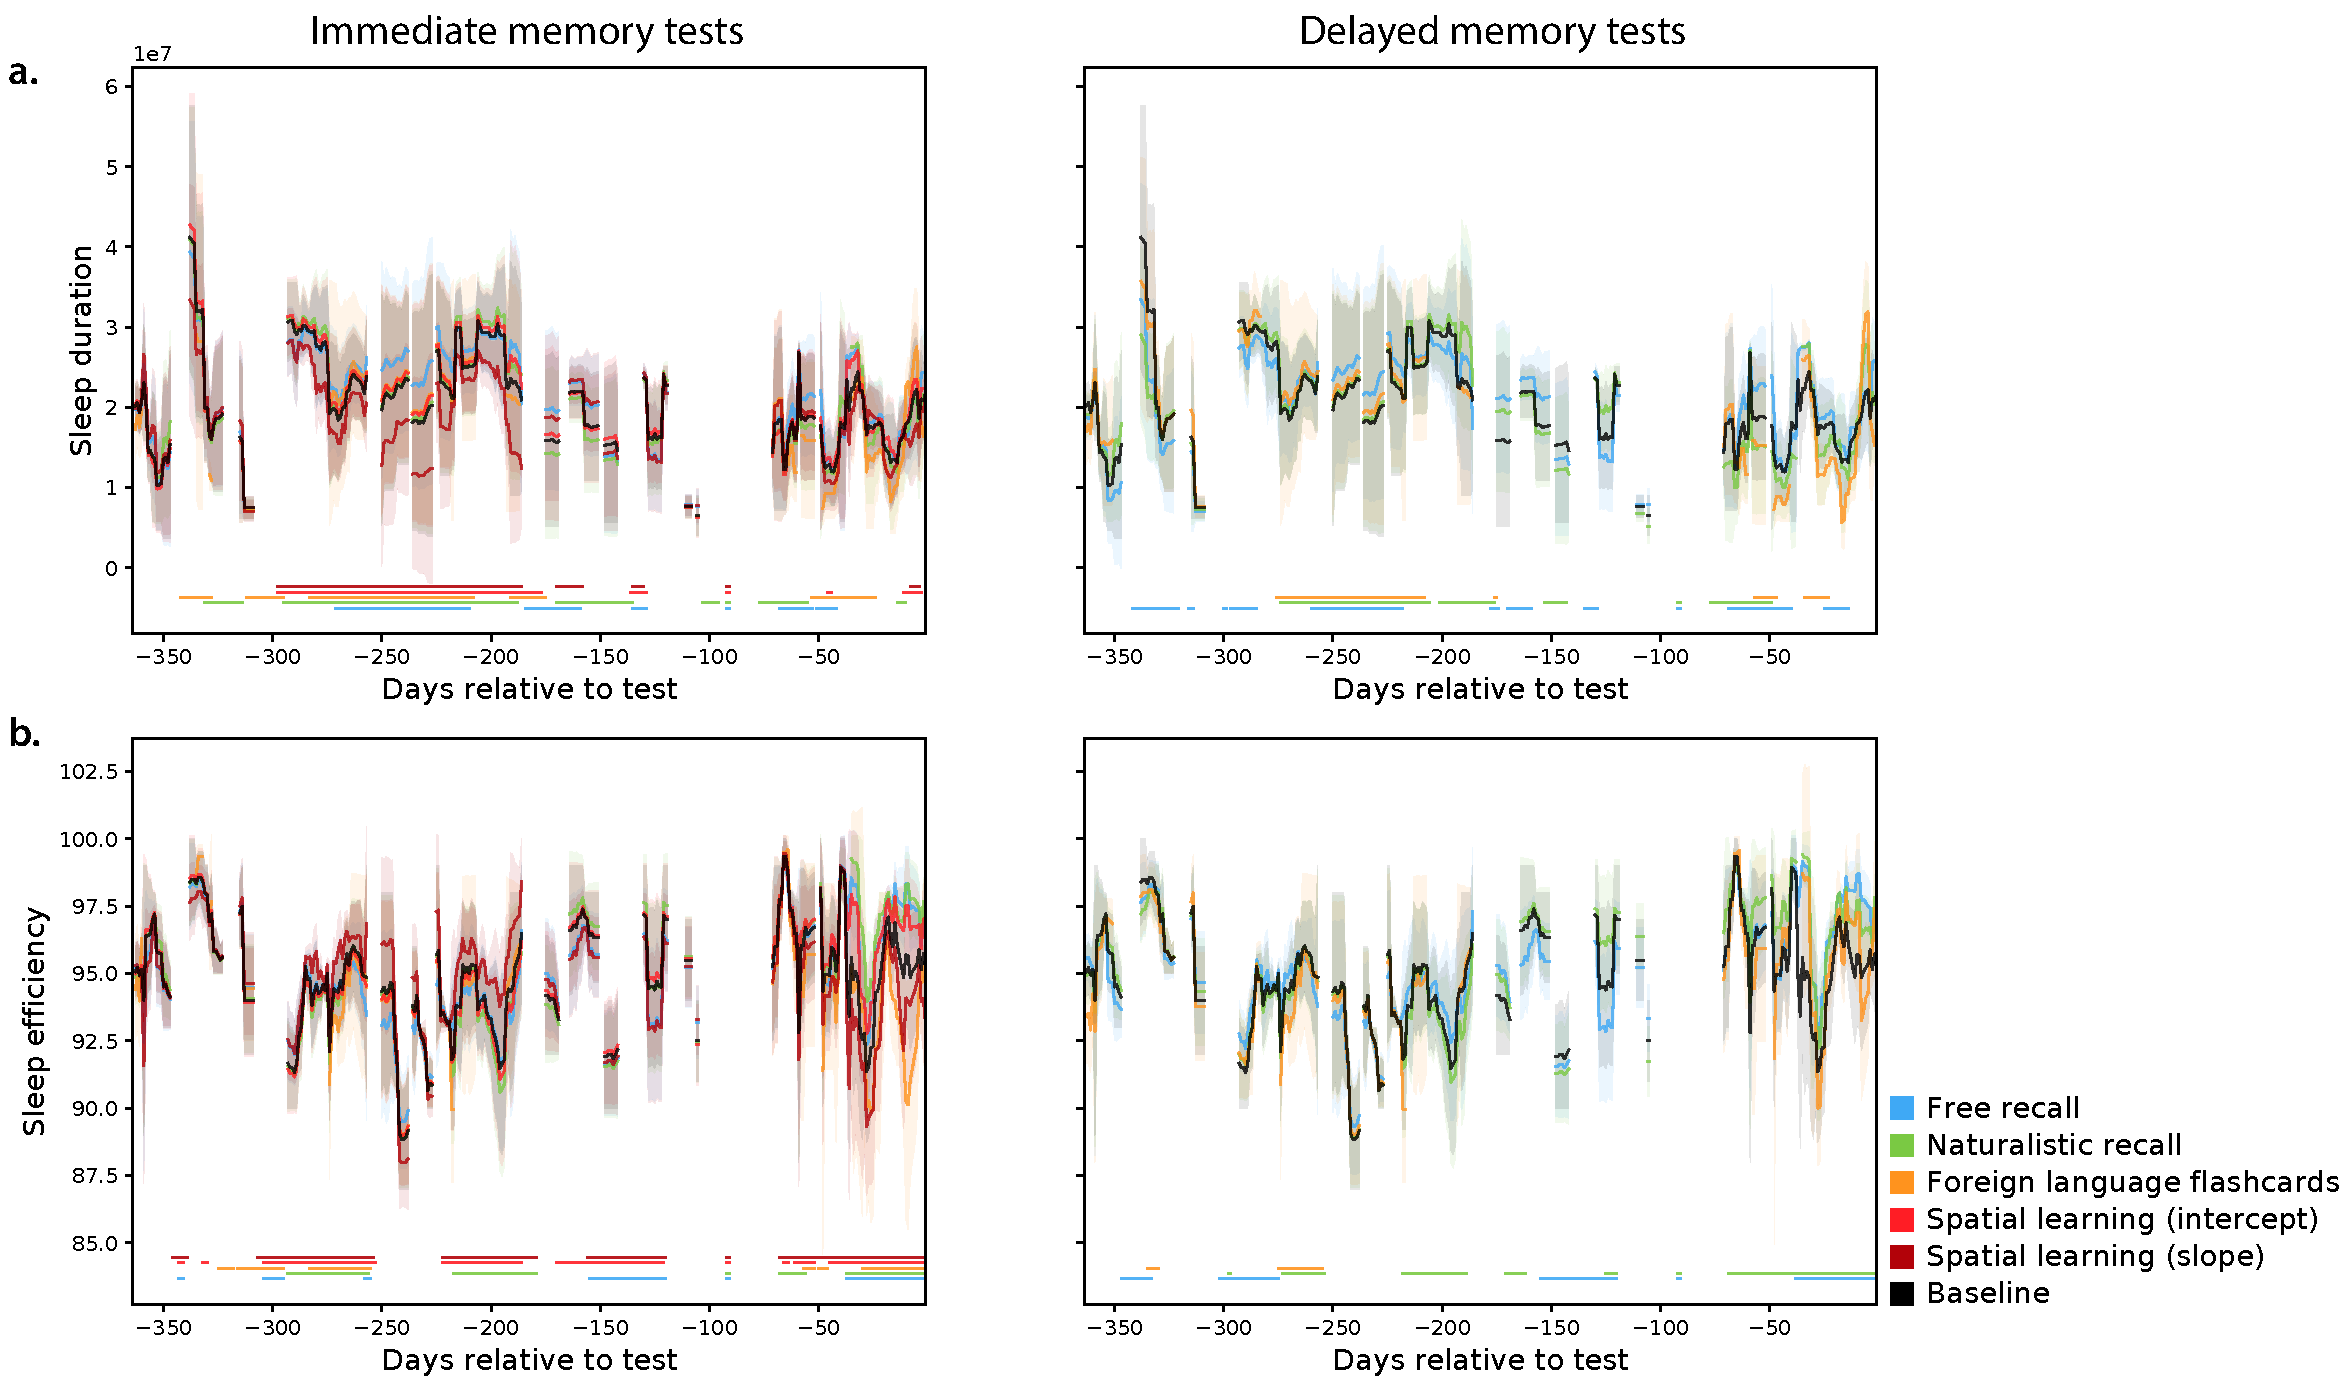
\includegraphics[width=0.75\textwidth]{figs/weighted_timecourse_sleep}
\caption{\textbf{History of sleep efficiency and duration weighted by
    behavioral performance.}}
\label{fig:sleep_timecourse}
\end{figure}

\begin{sidewaysfigure}[p]
  \centering
  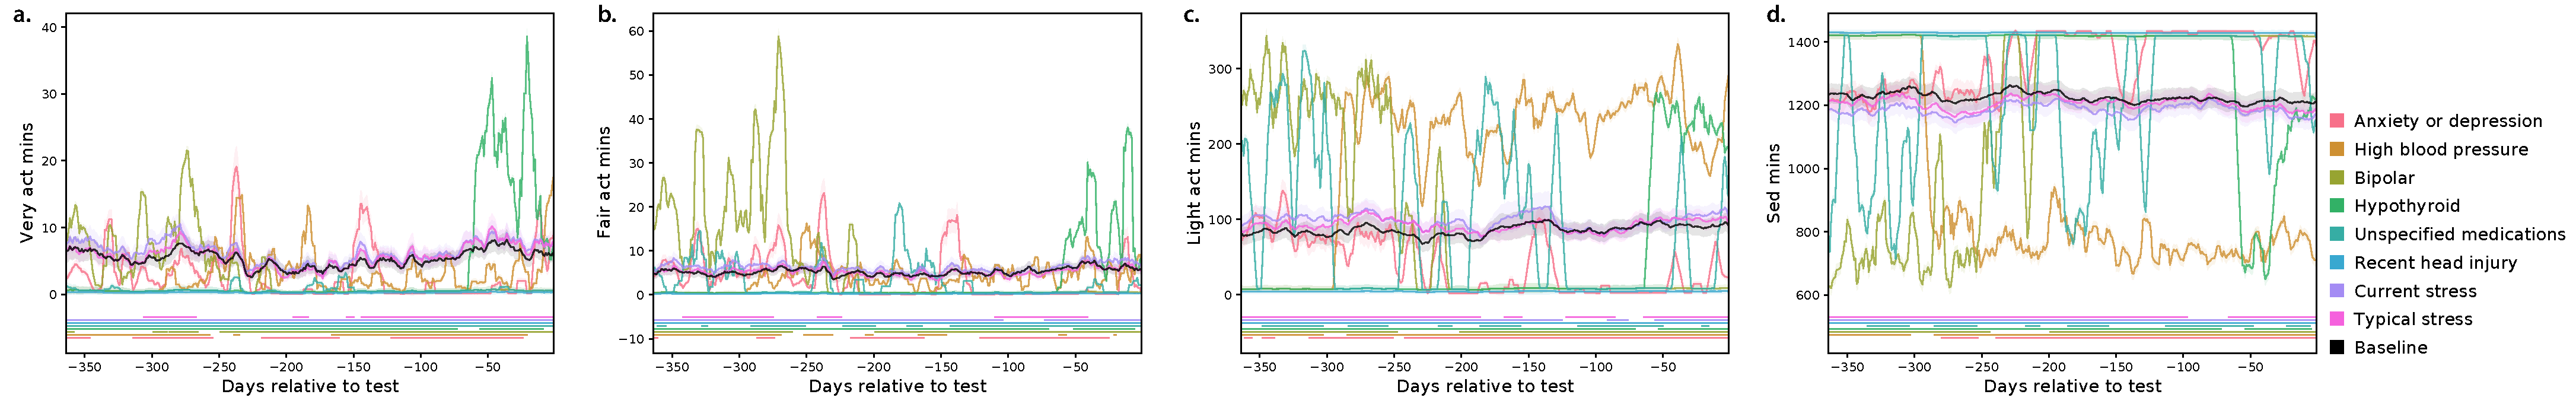
\includegraphics[width=0.75\textwidth]{figs/weighted_timecourse_activity_MH}
\caption{\textbf{History of fitness activity levels weighted by
    mental health factors.}}
\label{fig:activity_timecourse_MH}
\end{sidewaysfigure}

\begin{sidewaysfigure}[p]
  \centering
  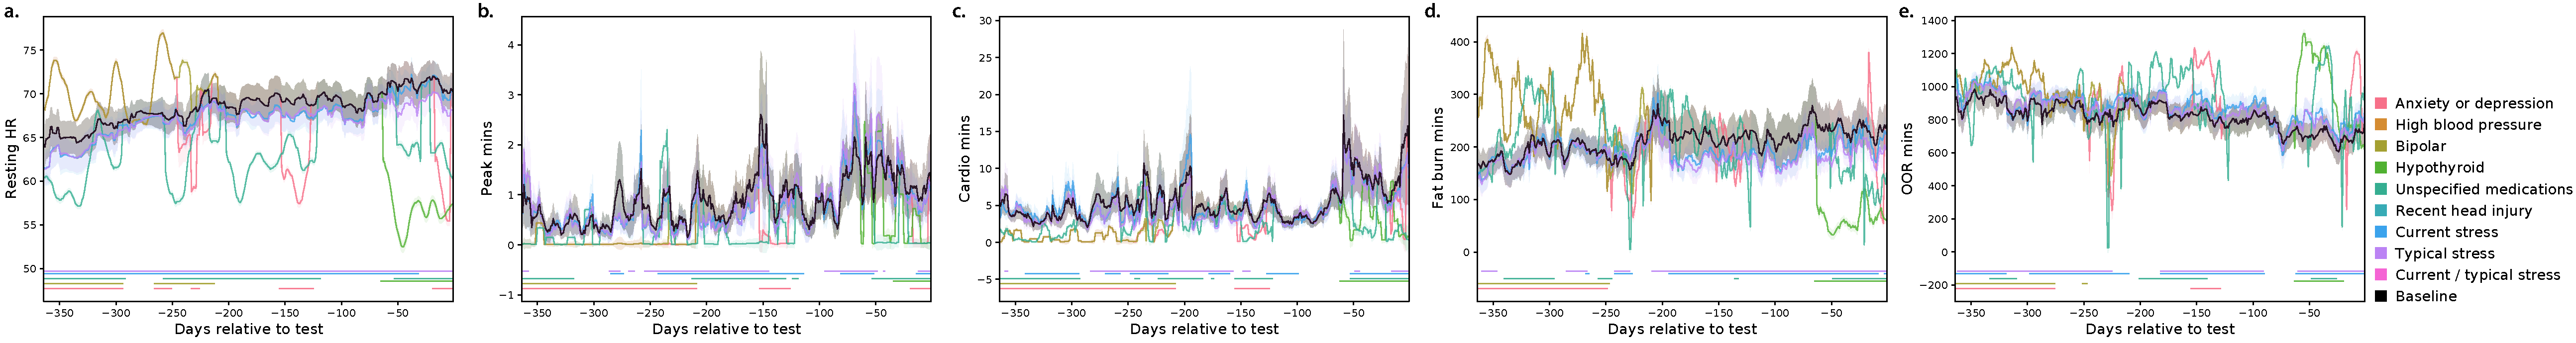
\includegraphics[width=\textwidth]{figs/weighted_timecourse_HR_MH}
\caption{\textbf{History of cardiovascular activity weighted by
    mental health factors.}}
\label{fig:HR_timecourse_MH}
  \end{sidewaysfigure}

\begin{figure}[p]
  \centering
  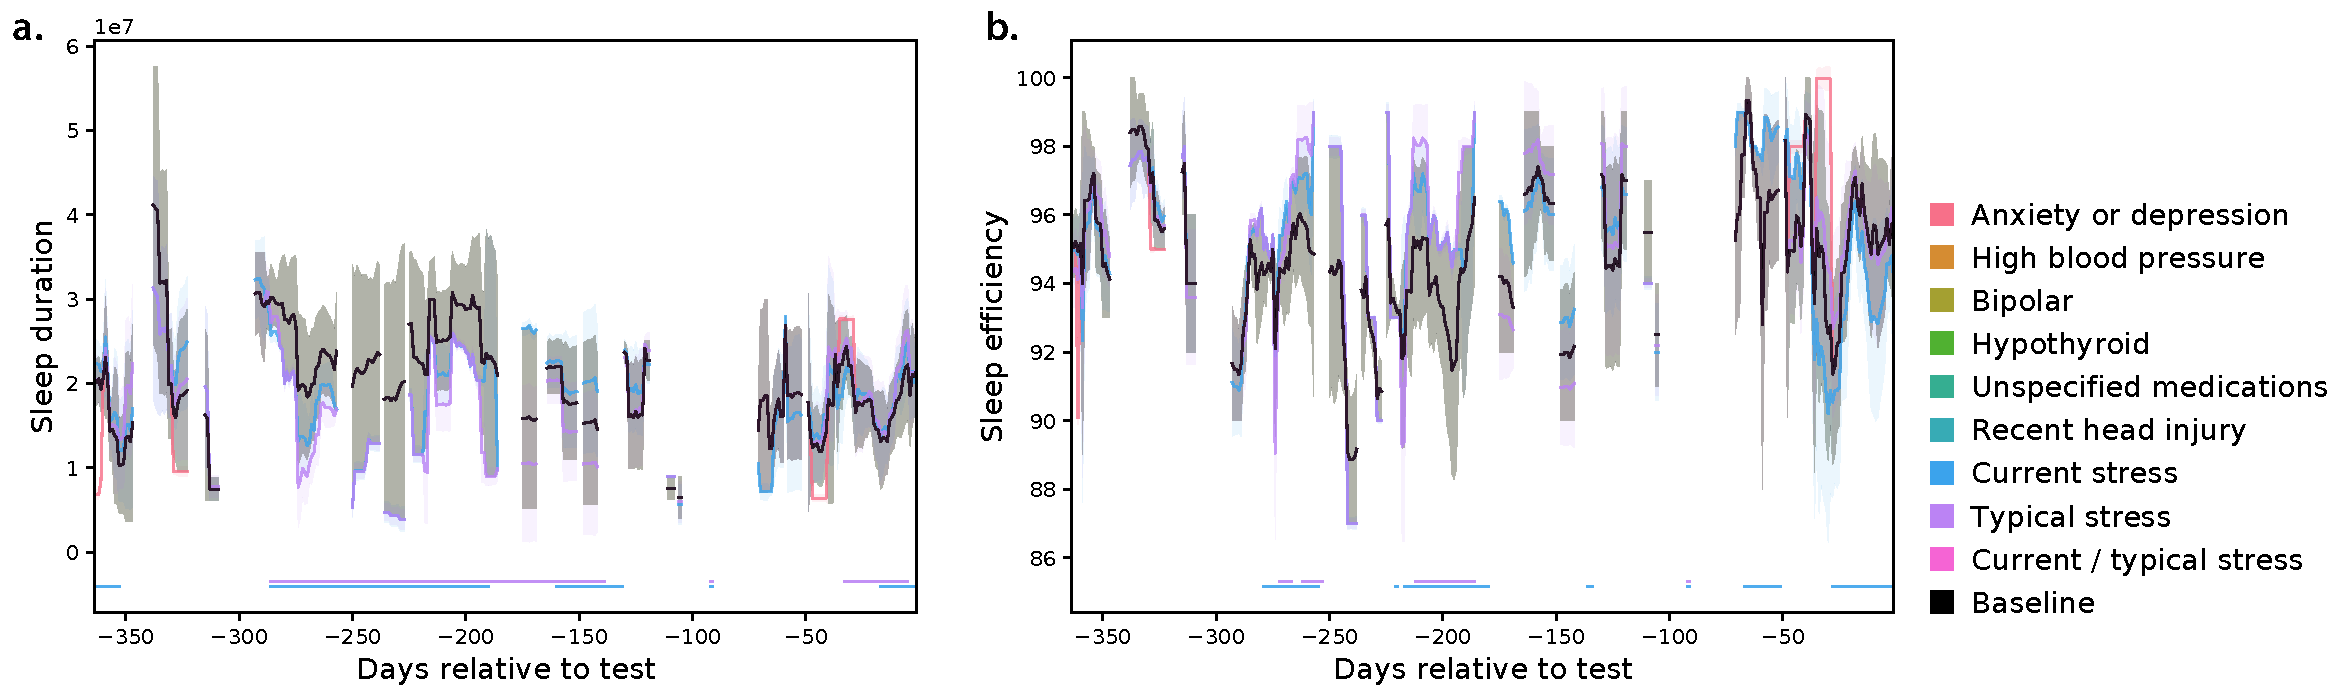
\includegraphics[width=0.75\textwidth]{figs/weighted_timecourse_sleep_MH}
\caption{\textbf{History of sleep efficiency and duration weighted by
    mental health factors.}}
\label{fig:sleep_timecourse_MH}
  \end{figure}

\bibliographystyle{apa}
\bibliography{/Users/jmanning/CDL-bibliography/cdl}
\end{document}
